\documentclass[twoside]{book}

% Packages required by doxygen
\usepackage{fixltx2e}
\usepackage{calc}
\usepackage{doxygen}
\usepackage{graphicx}
\usepackage[utf8]{inputenc}
\usepackage{makeidx}
\usepackage{multicol}
\usepackage{multirow}
\PassOptionsToPackage{warn}{textcomp}
\usepackage{textcomp}
\usepackage[nointegrals]{wasysym}
\usepackage[table]{xcolor}

% Font selection
\usepackage[T1]{fontenc}
\usepackage{mathptmx}
\usepackage[scaled=.90]{helvet}
\usepackage{courier}
\usepackage{amssymb}
\usepackage{sectsty}
\renewcommand{\familydefault}{\sfdefault}
\allsectionsfont{%
  \fontseries{bc}\selectfont%
  \color{darkgray}%
}
\renewcommand{\DoxyLabelFont}{%
  \fontseries{bc}\selectfont%
  \color{darkgray}%
}
\newcommand{\+}{\discretionary{\mbox{\scriptsize$\hookleftarrow$}}{}{}}

% Page & text layout
\usepackage{geometry}
\geometry{%
  a4paper,%
  top=2.5cm,%
  bottom=2.5cm,%
  left=2.5cm,%
  right=2.5cm%
}
\tolerance=750
\hfuzz=15pt
\hbadness=750
\setlength{\emergencystretch}{15pt}
\setlength{\parindent}{0cm}
\setlength{\parskip}{0.2cm}
\makeatletter
\renewcommand{\paragraph}{%
  \@startsection{paragraph}{4}{0ex}{-1.0ex}{1.0ex}{%
    \normalfont\normalsize\bfseries\SS@parafont%
  }%
}
\renewcommand{\subparagraph}{%
  \@startsection{subparagraph}{5}{0ex}{-1.0ex}{1.0ex}{%
    \normalfont\normalsize\bfseries\SS@subparafont%
  }%
}
\makeatother

% Headers & footers
\usepackage{fancyhdr}
\pagestyle{fancyplain}
\fancyhead[LE]{\fancyplain{}{\bfseries\thepage}}
\fancyhead[CE]{\fancyplain{}{}}
\fancyhead[RE]{\fancyplain{}{\bfseries\leftmark}}
\fancyhead[LO]{\fancyplain{}{\bfseries\rightmark}}
\fancyhead[CO]{\fancyplain{}{}}
\fancyhead[RO]{\fancyplain{}{\bfseries\thepage}}
\fancyfoot[LE]{\fancyplain{}{}}
\fancyfoot[CE]{\fancyplain{}{}}
\fancyfoot[RE]{\fancyplain{}{\bfseries\scriptsize Generated on Fri Jan 23 2015 09\+:39\+:30 for Setup by Doxygen }}
\fancyfoot[LO]{\fancyplain{}{\bfseries\scriptsize Generated on Fri Jan 23 2015 09\+:39\+:30 for Setup by Doxygen }}
\fancyfoot[CO]{\fancyplain{}{}}
\fancyfoot[RO]{\fancyplain{}{}}
\renewcommand{\footrulewidth}{0.4pt}
\renewcommand{\chaptermark}[1]{%
  \markboth{#1}{}%
}
\renewcommand{\sectionmark}[1]{%
  \markright{\thesection\ #1}%
}

% Indices & bibliography
\usepackage{natbib}
\usepackage[titles]{tocloft}
\setcounter{tocdepth}{3}
\setcounter{secnumdepth}{5}
\makeindex

% Hyperlinks (required, but should be loaded last)
\usepackage{ifpdf}
\ifpdf
  \usepackage[pdftex,pagebackref=true]{hyperref}
\else
  \usepackage[ps2pdf,pagebackref=true]{hyperref}
\fi
\hypersetup{%
  colorlinks=true,%
  linkcolor=blue,%
  citecolor=blue,%
  unicode%
}

% Custom commands
\newcommand{\clearemptydoublepage}{%
  \newpage{\pagestyle{empty}\cleardoublepage}%
}


%===== C O N T E N T S =====

\begin{document}

% Titlepage & ToC
\hypersetup{pageanchor=false,
             bookmarks=true,
             bookmarksnumbered=true,
             pdfencoding=unicode
            }
\pagenumbering{roman}
\begin{titlepage}
\vspace*{7cm}
\begin{center}%
{\Large Setup \\[1ex]\large 2 }\\
\vspace*{1cm}
{\large Generated by Doxygen 1.8.8}\\
\vspace*{0.5cm}
{\small Fri Jan 23 2015 09:39:30}\\
\end{center}
\end{titlepage}
\clearemptydoublepage
\tableofcontents
\clearemptydoublepage
\pagenumbering{arabic}
\hypersetup{pageanchor=true}

%--- Begin generated contents ---
\chapter{Class Index}
\section{Class List}
Here are the classes, structs, unions and interfaces with brief descriptions\+:\begin{DoxyCompactList}
\item\contentsline{section}{\hyperlink{class_c_class}{C\+Class} }{\pageref{class_c_class}}{}
\item\contentsline{section}{\hyperlink{class_c_class_manager}{C\+Class\+Manager} }{\pageref{class_c_class_manager}}{}
\item\contentsline{section}{\hyperlink{class_c_files_finder}{C\+Files\+Finder} }{\pageref{class_c_files_finder}}{}
\item\contentsline{section}{\hyperlink{struct_c_files_finder_1_1_s_file}{C\+Files\+Finder\+::\+S\+File} }{\pageref{struct_c_files_finder_1_1_s_file}}{}
\item\contentsline{section}{\hyperlink{struct_c_class_1_1_s_function}{C\+Class\+::\+S\+Function} }{\pageref{struct_c_class_1_1_s_function}}{}
\end{DoxyCompactList}

\chapter{File Index}
\section{File List}
Here is a list of all files with brief descriptions\+:\begin{DoxyCompactList}
\item\contentsline{section}{diagrams/\hyperlink{_class_8cpp}{Class.\+cpp} }{\pageref{_class_8cpp}}{}
\item\contentsline{section}{diagrams/\hyperlink{_class_8h}{Class.\+h} }{\pageref{_class_8h}}{}
\item\contentsline{section}{diagrams/\hyperlink{_class_manager_8cpp}{Class\+Manager.\+cpp} }{\pageref{_class_manager_8cpp}}{}
\item\contentsline{section}{diagrams/\hyperlink{_class_manager_8h}{Class\+Manager.\+h} }{\pageref{_class_manager_8h}}{}
\item\contentsline{section}{diagrams/\hyperlink{diagrams_8cpp}{diagrams.\+cpp} }{\pageref{diagrams_8cpp}}{}
\item\contentsline{section}{diagrams/\hyperlink{_files_finder_8cpp}{Files\+Finder.\+cpp} }{\pageref{_files_finder_8cpp}}{}
\item\contentsline{section}{diagrams/\hyperlink{_files_finder_8h}{Files\+Finder.\+h} }{\pageref{_files_finder_8h}}{}
\item\contentsline{section}{diagrams/\hyperlink{stdafx_8cpp}{stdafx.\+cpp} }{\pageref{stdafx_8cpp}}{}
\item\contentsline{section}{diagrams/\hyperlink{stdafx_8h}{stdafx.\+h} }{\pageref{stdafx_8h}}{}
\item\contentsline{section}{diagrams/\hyperlink{targetver_8h}{targetver.\+h} }{\pageref{targetver_8h}}{}
\end{DoxyCompactList}

\chapter{Class Documentation}
\hypertarget{class_c_class}{\section{C\+Class Class Reference}
\label{class_c_class}\index{C\+Class@{C\+Class}}
}


{\ttfamily \#include $<$Class.\+h$>$}



Collaboration diagram for C\+Class\+:
\nopagebreak
\begin{figure}[H]
\begin{center}
\leavevmode
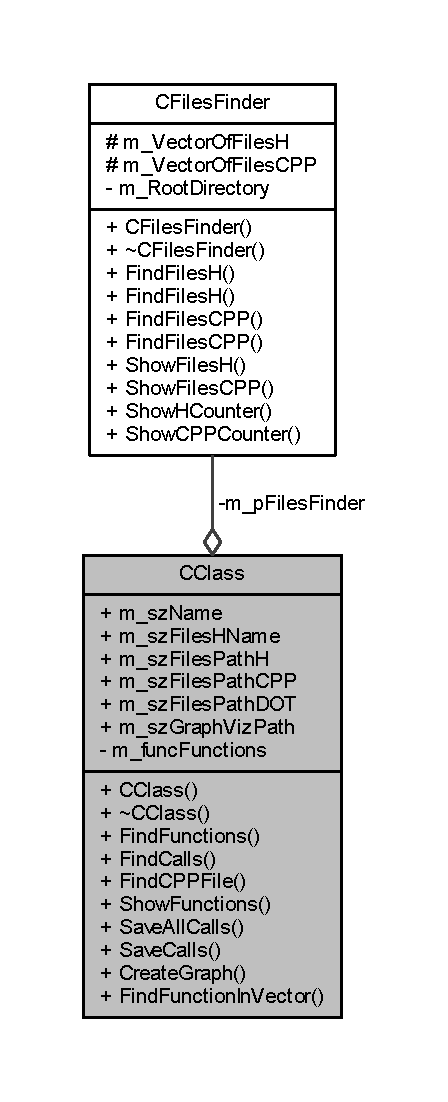
\includegraphics[width=215pt]{class_c_class__coll__graph}
\end{center}
\end{figure}
\subsection*{Classes}
\begin{DoxyCompactItemize}
\item 
struct \hyperlink{struct_c_class_1_1_s_function}{S\+Function}
\end{DoxyCompactItemize}
\subsection*{Public Member Functions}
\begin{DoxyCompactItemize}
\item 
\hyperlink{class_c_class_a9d835b0d9c9cbc2abb5859f5839cc768}{C\+Class} (string a\+\_\+sz\+Name, string a\+\_\+sz\+Files\+Path\+H, \hyperlink{class_c_files_finder}{C\+Files\+Finder} $\ast$a\+\_\+p\+Files\+Finder)
\item 
\hyperlink{class_c_class_ab3bd712c48cc40f0e8b1cebe714dd2ed}{$\sim$\+C\+Class} ()
\item 
bool \hyperlink{class_c_class_a23774d2a60493cba0f87f2ccce1112e9}{Find\+Functions} ()
\item 
bool \hyperlink{class_c_class_a0a6b7022064d70e613755b46f71bfb3e}{Find\+Calls} ()
\item 
bool \hyperlink{class_c_class_a60f873762e2cf01154d819e963983f16}{Find\+C\+P\+P\+File} ()
\item 
void \hyperlink{class_c_class_aa4a34bb2e8c824dda17c8a12569de25a}{Show\+Functions} ()
\item 
bool \hyperlink{class_c_class_a1a1b258d491f553ba7db631a9a7ed9b5}{Save\+All\+Calls} ()
\item 
bool \hyperlink{class_c_class_aaae438dee1363c920c18bd96a29220fd}{Save\+Calls} (string a\+\_\+sz\+Function\+Name)
\item 
bool \hyperlink{class_c_class_a7fe0dadc365b5a396e5d14938061a699}{Create\+Graph} ()
\item 
int \hyperlink{class_c_class_a8c2b52a935357403b2599650f8d0cd37}{Find\+Function\+In\+Vector} (string a\+\_\+sz\+Function\+Name)
\end{DoxyCompactItemize}
\subsection*{Public Attributes}
\begin{DoxyCompactItemize}
\item 
string \hyperlink{class_c_class_ae7f5bac3dd30935df8d31dacacfea3e2}{m\+\_\+sz\+Name}
\item 
string \hyperlink{class_c_class_a15cee6cfe5a893a807799fb33d53db99}{m\+\_\+sz\+Files\+H\+Name}
\item 
string \hyperlink{class_c_class_a590754a9bdd5a6fc0104378da2fb7891}{m\+\_\+sz\+Files\+Path\+H}
\item 
string \hyperlink{class_c_class_a684985105ee38e9face97c886bcb86ce}{m\+\_\+sz\+Files\+Path\+C\+P\+P}
\item 
string \hyperlink{class_c_class_a4cf97b0cde501346ac139deaeab2573a}{m\+\_\+sz\+Files\+Path\+D\+O\+T}
\item 
const string \hyperlink{class_c_class_a8ee7eb6ac6ebd9f4b31324f9daeb07c2}{m\+\_\+sz\+Graph\+Viz\+Path} = \char`\"{}C\+:\textbackslash{}\textbackslash{}\+Users\textbackslash{}\textbackslash{}ciosebar\textbackslash{}\textbackslash{}\+Desktop\textbackslash{}\textbackslash{}graphviz-\/2.\+38\textbackslash{}\textbackslash{}release\textbackslash{}\textbackslash{}bin\textbackslash{}\textbackslash{}\char`\"{}
\end{DoxyCompactItemize}
\subsection*{Private Attributes}
\begin{DoxyCompactItemize}
\item 
\hyperlink{class_c_files_finder}{C\+Files\+Finder} $\ast$ \hyperlink{class_c_class_a253ea247276cd6daeed278c17bebd67a}{m\+\_\+p\+Files\+Finder}
\item 
vector$<$ \hyperlink{struct_c_class_1_1_s_function}{S\+Function} $>$ \hyperlink{class_c_class_a1468409456184a03f237f28f6004a514}{m\+\_\+func\+Functions}
\end{DoxyCompactItemize}


\subsection{Constructor \& Destructor Documentation}
\hypertarget{class_c_class_a9d835b0d9c9cbc2abb5859f5839cc768}{\index{C\+Class@{C\+Class}!C\+Class@{C\+Class}}
\index{C\+Class@{C\+Class}!C\+Class@{C\+Class}}
\subsubsection[{C\+Class}]{\setlength{\rightskip}{0pt plus 5cm}C\+Class\+::\+C\+Class (
\begin{DoxyParamCaption}
\item[{string}]{a\+\_\+sz\+Name, }
\item[{string}]{a\+\_\+sz\+Files\+Path\+H, }
\item[{{\bf C\+Files\+Finder} $\ast$}]{a\+\_\+p\+Files\+Finder}
\end{DoxyParamCaption}
)}}\label{class_c_class_a9d835b0d9c9cbc2abb5859f5839cc768}
\hypertarget{class_c_class_ab3bd712c48cc40f0e8b1cebe714dd2ed}{\index{C\+Class@{C\+Class}!````~C\+Class@{$\sim$\+C\+Class}}
\index{````~C\+Class@{$\sim$\+C\+Class}!C\+Class@{C\+Class}}
\subsubsection[{$\sim$\+C\+Class}]{\setlength{\rightskip}{0pt plus 5cm}C\+Class\+::$\sim$\+C\+Class (
\begin{DoxyParamCaption}
{}
\end{DoxyParamCaption}
)}}\label{class_c_class_ab3bd712c48cc40f0e8b1cebe714dd2ed}


\subsection{Member Function Documentation}
\hypertarget{class_c_class_a7fe0dadc365b5a396e5d14938061a699}{\index{C\+Class@{C\+Class}!Create\+Graph@{Create\+Graph}}
\index{Create\+Graph@{Create\+Graph}!C\+Class@{C\+Class}}
\subsubsection[{Create\+Graph}]{\setlength{\rightskip}{0pt plus 5cm}bool C\+Class\+::\+Create\+Graph (
\begin{DoxyParamCaption}
{}
\end{DoxyParamCaption}
)}}\label{class_c_class_a7fe0dadc365b5a396e5d14938061a699}
\hypertarget{class_c_class_a0a6b7022064d70e613755b46f71bfb3e}{\index{C\+Class@{C\+Class}!Find\+Calls@{Find\+Calls}}
\index{Find\+Calls@{Find\+Calls}!C\+Class@{C\+Class}}
\subsubsection[{Find\+Calls}]{\setlength{\rightskip}{0pt plus 5cm}bool C\+Class\+::\+Find\+Calls (
\begin{DoxyParamCaption}
{}
\end{DoxyParamCaption}
)}}\label{class_c_class_a0a6b7022064d70e613755b46f71bfb3e}
\hypertarget{class_c_class_a60f873762e2cf01154d819e963983f16}{\index{C\+Class@{C\+Class}!Find\+C\+P\+P\+File@{Find\+C\+P\+P\+File}}
\index{Find\+C\+P\+P\+File@{Find\+C\+P\+P\+File}!C\+Class@{C\+Class}}
\subsubsection[{Find\+C\+P\+P\+File}]{\setlength{\rightskip}{0pt plus 5cm}bool C\+Class\+::\+Find\+C\+P\+P\+File (
\begin{DoxyParamCaption}
{}
\end{DoxyParamCaption}
)}}\label{class_c_class_a60f873762e2cf01154d819e963983f16}
\hypertarget{class_c_class_a8c2b52a935357403b2599650f8d0cd37}{\index{C\+Class@{C\+Class}!Find\+Function\+In\+Vector@{Find\+Function\+In\+Vector}}
\index{Find\+Function\+In\+Vector@{Find\+Function\+In\+Vector}!C\+Class@{C\+Class}}
\subsubsection[{Find\+Function\+In\+Vector}]{\setlength{\rightskip}{0pt plus 5cm}int C\+Class\+::\+Find\+Function\+In\+Vector (
\begin{DoxyParamCaption}
\item[{string}]{a\+\_\+sz\+Function\+Name}
\end{DoxyParamCaption}
)}}\label{class_c_class_a8c2b52a935357403b2599650f8d0cd37}
\hypertarget{class_c_class_a23774d2a60493cba0f87f2ccce1112e9}{\index{C\+Class@{C\+Class}!Find\+Functions@{Find\+Functions}}
\index{Find\+Functions@{Find\+Functions}!C\+Class@{C\+Class}}
\subsubsection[{Find\+Functions}]{\setlength{\rightskip}{0pt plus 5cm}bool C\+Class\+::\+Find\+Functions (
\begin{DoxyParamCaption}
{}
\end{DoxyParamCaption}
)}}\label{class_c_class_a23774d2a60493cba0f87f2ccce1112e9}
\hypertarget{class_c_class_a1a1b258d491f553ba7db631a9a7ed9b5}{\index{C\+Class@{C\+Class}!Save\+All\+Calls@{Save\+All\+Calls}}
\index{Save\+All\+Calls@{Save\+All\+Calls}!C\+Class@{C\+Class}}
\subsubsection[{Save\+All\+Calls}]{\setlength{\rightskip}{0pt plus 5cm}bool C\+Class\+::\+Save\+All\+Calls (
\begin{DoxyParamCaption}
{}
\end{DoxyParamCaption}
)}}\label{class_c_class_a1a1b258d491f553ba7db631a9a7ed9b5}
\hypertarget{class_c_class_aaae438dee1363c920c18bd96a29220fd}{\index{C\+Class@{C\+Class}!Save\+Calls@{Save\+Calls}}
\index{Save\+Calls@{Save\+Calls}!C\+Class@{C\+Class}}
\subsubsection[{Save\+Calls}]{\setlength{\rightskip}{0pt plus 5cm}bool C\+Class\+::\+Save\+Calls (
\begin{DoxyParamCaption}
\item[{string}]{a\+\_\+sz\+Function\+Name}
\end{DoxyParamCaption}
)}}\label{class_c_class_aaae438dee1363c920c18bd96a29220fd}
\hypertarget{class_c_class_aa4a34bb2e8c824dda17c8a12569de25a}{\index{C\+Class@{C\+Class}!Show\+Functions@{Show\+Functions}}
\index{Show\+Functions@{Show\+Functions}!C\+Class@{C\+Class}}
\subsubsection[{Show\+Functions}]{\setlength{\rightskip}{0pt plus 5cm}void C\+Class\+::\+Show\+Functions (
\begin{DoxyParamCaption}
{}
\end{DoxyParamCaption}
)}}\label{class_c_class_aa4a34bb2e8c824dda17c8a12569de25a}


\subsection{Member Data Documentation}
\hypertarget{class_c_class_a1468409456184a03f237f28f6004a514}{\index{C\+Class@{C\+Class}!m\+\_\+func\+Functions@{m\+\_\+func\+Functions}}
\index{m\+\_\+func\+Functions@{m\+\_\+func\+Functions}!C\+Class@{C\+Class}}
\subsubsection[{m\+\_\+func\+Functions}]{\setlength{\rightskip}{0pt plus 5cm}vector$<${\bf S\+Function}$>$ C\+Class\+::m\+\_\+func\+Functions\hspace{0.3cm}{\ttfamily [private]}}}\label{class_c_class_a1468409456184a03f237f28f6004a514}
\hypertarget{class_c_class_a253ea247276cd6daeed278c17bebd67a}{\index{C\+Class@{C\+Class}!m\+\_\+p\+Files\+Finder@{m\+\_\+p\+Files\+Finder}}
\index{m\+\_\+p\+Files\+Finder@{m\+\_\+p\+Files\+Finder}!C\+Class@{C\+Class}}
\subsubsection[{m\+\_\+p\+Files\+Finder}]{\setlength{\rightskip}{0pt plus 5cm}{\bf C\+Files\+Finder}$\ast$ C\+Class\+::m\+\_\+p\+Files\+Finder\hspace{0.3cm}{\ttfamily [private]}}}\label{class_c_class_a253ea247276cd6daeed278c17bebd67a}
\hypertarget{class_c_class_a15cee6cfe5a893a807799fb33d53db99}{\index{C\+Class@{C\+Class}!m\+\_\+sz\+Files\+H\+Name@{m\+\_\+sz\+Files\+H\+Name}}
\index{m\+\_\+sz\+Files\+H\+Name@{m\+\_\+sz\+Files\+H\+Name}!C\+Class@{C\+Class}}
\subsubsection[{m\+\_\+sz\+Files\+H\+Name}]{\setlength{\rightskip}{0pt plus 5cm}string C\+Class\+::m\+\_\+sz\+Files\+H\+Name}}\label{class_c_class_a15cee6cfe5a893a807799fb33d53db99}
\hypertarget{class_c_class_a684985105ee38e9face97c886bcb86ce}{\index{C\+Class@{C\+Class}!m\+\_\+sz\+Files\+Path\+C\+P\+P@{m\+\_\+sz\+Files\+Path\+C\+P\+P}}
\index{m\+\_\+sz\+Files\+Path\+C\+P\+P@{m\+\_\+sz\+Files\+Path\+C\+P\+P}!C\+Class@{C\+Class}}
\subsubsection[{m\+\_\+sz\+Files\+Path\+C\+P\+P}]{\setlength{\rightskip}{0pt plus 5cm}string C\+Class\+::m\+\_\+sz\+Files\+Path\+C\+P\+P}}\label{class_c_class_a684985105ee38e9face97c886bcb86ce}
\hypertarget{class_c_class_a4cf97b0cde501346ac139deaeab2573a}{\index{C\+Class@{C\+Class}!m\+\_\+sz\+Files\+Path\+D\+O\+T@{m\+\_\+sz\+Files\+Path\+D\+O\+T}}
\index{m\+\_\+sz\+Files\+Path\+D\+O\+T@{m\+\_\+sz\+Files\+Path\+D\+O\+T}!C\+Class@{C\+Class}}
\subsubsection[{m\+\_\+sz\+Files\+Path\+D\+O\+T}]{\setlength{\rightskip}{0pt plus 5cm}string C\+Class\+::m\+\_\+sz\+Files\+Path\+D\+O\+T}}\label{class_c_class_a4cf97b0cde501346ac139deaeab2573a}
\hypertarget{class_c_class_a590754a9bdd5a6fc0104378da2fb7891}{\index{C\+Class@{C\+Class}!m\+\_\+sz\+Files\+Path\+H@{m\+\_\+sz\+Files\+Path\+H}}
\index{m\+\_\+sz\+Files\+Path\+H@{m\+\_\+sz\+Files\+Path\+H}!C\+Class@{C\+Class}}
\subsubsection[{m\+\_\+sz\+Files\+Path\+H}]{\setlength{\rightskip}{0pt plus 5cm}string C\+Class\+::m\+\_\+sz\+Files\+Path\+H}}\label{class_c_class_a590754a9bdd5a6fc0104378da2fb7891}
\hypertarget{class_c_class_a8ee7eb6ac6ebd9f4b31324f9daeb07c2}{\index{C\+Class@{C\+Class}!m\+\_\+sz\+Graph\+Viz\+Path@{m\+\_\+sz\+Graph\+Viz\+Path}}
\index{m\+\_\+sz\+Graph\+Viz\+Path@{m\+\_\+sz\+Graph\+Viz\+Path}!C\+Class@{C\+Class}}
\subsubsection[{m\+\_\+sz\+Graph\+Viz\+Path}]{\setlength{\rightskip}{0pt plus 5cm}const string C\+Class\+::m\+\_\+sz\+Graph\+Viz\+Path = \char`\"{}C\+:\textbackslash{}\textbackslash{}\+Users\textbackslash{}\textbackslash{}ciosebar\textbackslash{}\textbackslash{}\+Desktop\textbackslash{}\textbackslash{}graphviz-\/2.\+38\textbackslash{}\textbackslash{}release\textbackslash{}\textbackslash{}bin\textbackslash{}\textbackslash{}\char`\"{}}}\label{class_c_class_a8ee7eb6ac6ebd9f4b31324f9daeb07c2}
\hypertarget{class_c_class_ae7f5bac3dd30935df8d31dacacfea3e2}{\index{C\+Class@{C\+Class}!m\+\_\+sz\+Name@{m\+\_\+sz\+Name}}
\index{m\+\_\+sz\+Name@{m\+\_\+sz\+Name}!C\+Class@{C\+Class}}
\subsubsection[{m\+\_\+sz\+Name}]{\setlength{\rightskip}{0pt plus 5cm}string C\+Class\+::m\+\_\+sz\+Name}}\label{class_c_class_ae7f5bac3dd30935df8d31dacacfea3e2}


The documentation for this class was generated from the following files\+:\begin{DoxyCompactItemize}
\item 
diagrams/\hyperlink{_class_8h}{Class.\+h}\item 
diagrams/\hyperlink{_class_8cpp}{Class.\+cpp}\end{DoxyCompactItemize}

\hypertarget{class_c_class_manager}{\section{C\+Class\+Manager Class Reference}
\label{class_c_class_manager}\index{C\+Class\+Manager@{C\+Class\+Manager}}
}


{\ttfamily \#include $<$Class\+Manager.\+h$>$}



Collaboration diagram for C\+Class\+Manager\+:
\nopagebreak
\begin{figure}[H]
\begin{center}
\leavevmode
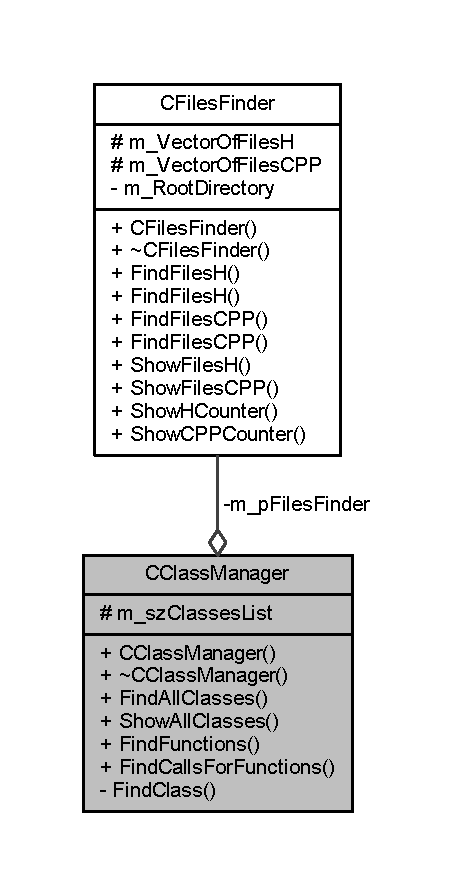
\includegraphics[width=218pt]{class_c_class_manager__coll__graph}
\end{center}
\end{figure}
\subsection*{Public Member Functions}
\begin{DoxyCompactItemize}
\item 
\hyperlink{class_c_class_manager_a3c3a80c00e5cf6c1698d5d4ee694db5c}{C\+Class\+Manager} (\hyperlink{class_c_files_finder}{C\+Files\+Finder} $\ast$a\+\_\+p\+Files\+Finder)
\item 
\hyperlink{class_c_class_manager_adac08f657e5d8965166a561f58e13b7d}{$\sim$\+C\+Class\+Manager} ()
\item 
bool \hyperlink{class_c_class_manager_a6fe927748562e26c60da40b7b54a35c8}{Find\+All\+Classes} ()
\item 
void \hyperlink{class_c_class_manager_a7a5bd390df1b4100f452d56f94cadf24}{Show\+All\+Classes} ()
\item 
bool \hyperlink{class_c_class_manager_a1df8fae08901fc20f20e7f7f5120d267}{Find\+Functions} ()
\item 
bool \hyperlink{class_c_class_manager_a7a44afac10c69c87860c65040b23b57a}{Find\+Calls\+For\+Functions} ()
\end{DoxyCompactItemize}
\subsection*{Protected Attributes}
\begin{DoxyCompactItemize}
\item 
std\+::vector$<$ \hyperlink{class_c_class}{C\+Class} $>$ \hyperlink{class_c_class_manager_acbcada64d77a7fa05c8c6ffadcf730db}{m\+\_\+sz\+Classes\+List}
\end{DoxyCompactItemize}
\subsection*{Private Member Functions}
\begin{DoxyCompactItemize}
\item 
bool \hyperlink{class_c_class_manager_a1db9b102548bc1b9becf44031d5c3937}{Find\+Class} (string a\+\_\+sz\+Files\+Path)
\end{DoxyCompactItemize}
\subsection*{Private Attributes}
\begin{DoxyCompactItemize}
\item 
\hyperlink{class_c_files_finder}{C\+Files\+Finder} $\ast$ \hyperlink{class_c_class_manager_a6ea255cab18dff35dd07390af7776675}{m\+\_\+p\+Files\+Finder}
\end{DoxyCompactItemize}


\subsection{Constructor \& Destructor Documentation}
\hypertarget{class_c_class_manager_a3c3a80c00e5cf6c1698d5d4ee694db5c}{\index{C\+Class\+Manager@{C\+Class\+Manager}!C\+Class\+Manager@{C\+Class\+Manager}}
\index{C\+Class\+Manager@{C\+Class\+Manager}!C\+Class\+Manager@{C\+Class\+Manager}}
\subsubsection[{C\+Class\+Manager}]{\setlength{\rightskip}{0pt plus 5cm}C\+Class\+Manager\+::\+C\+Class\+Manager (
\begin{DoxyParamCaption}
\item[{{\bf C\+Files\+Finder} $\ast$}]{a\+\_\+p\+Files\+Finder}
\end{DoxyParamCaption}
)}}\label{class_c_class_manager_a3c3a80c00e5cf6c1698d5d4ee694db5c}
\hypertarget{class_c_class_manager_adac08f657e5d8965166a561f58e13b7d}{\index{C\+Class\+Manager@{C\+Class\+Manager}!````~C\+Class\+Manager@{$\sim$\+C\+Class\+Manager}}
\index{````~C\+Class\+Manager@{$\sim$\+C\+Class\+Manager}!C\+Class\+Manager@{C\+Class\+Manager}}
\subsubsection[{$\sim$\+C\+Class\+Manager}]{\setlength{\rightskip}{0pt plus 5cm}C\+Class\+Manager\+::$\sim$\+C\+Class\+Manager (
\begin{DoxyParamCaption}
{}
\end{DoxyParamCaption}
)}}\label{class_c_class_manager_adac08f657e5d8965166a561f58e13b7d}


\subsection{Member Function Documentation}
\hypertarget{class_c_class_manager_a6fe927748562e26c60da40b7b54a35c8}{\index{C\+Class\+Manager@{C\+Class\+Manager}!Find\+All\+Classes@{Find\+All\+Classes}}
\index{Find\+All\+Classes@{Find\+All\+Classes}!C\+Class\+Manager@{C\+Class\+Manager}}
\subsubsection[{Find\+All\+Classes}]{\setlength{\rightskip}{0pt plus 5cm}bool C\+Class\+Manager\+::\+Find\+All\+Classes (
\begin{DoxyParamCaption}
{}
\end{DoxyParamCaption}
)}}\label{class_c_class_manager_a6fe927748562e26c60da40b7b54a35c8}


Here is the call graph for this function\+:
\nopagebreak
\begin{figure}[H]
\begin{center}
\leavevmode
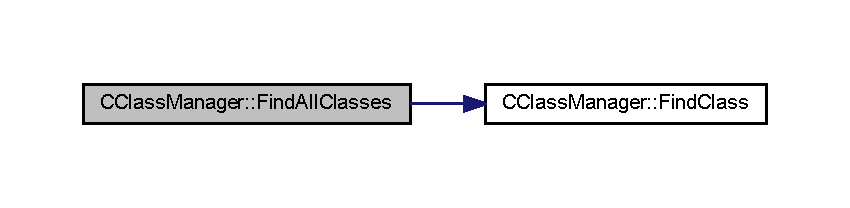
\includegraphics[width=350pt]{class_c_class_manager_a6fe927748562e26c60da40b7b54a35c8_cgraph}
\end{center}
\end{figure}




Here is the caller graph for this function\+:
\nopagebreak
\begin{figure}[H]
\begin{center}
\leavevmode
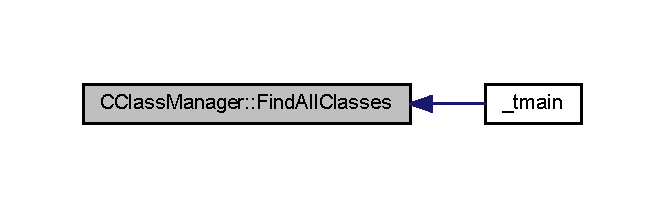
\includegraphics[width=319pt]{class_c_class_manager_a6fe927748562e26c60da40b7b54a35c8_icgraph}
\end{center}
\end{figure}


\hypertarget{class_c_class_manager_a7a44afac10c69c87860c65040b23b57a}{\index{C\+Class\+Manager@{C\+Class\+Manager}!Find\+Calls\+For\+Functions@{Find\+Calls\+For\+Functions}}
\index{Find\+Calls\+For\+Functions@{Find\+Calls\+For\+Functions}!C\+Class\+Manager@{C\+Class\+Manager}}
\subsubsection[{Find\+Calls\+For\+Functions}]{\setlength{\rightskip}{0pt plus 5cm}bool C\+Class\+Manager\+::\+Find\+Calls\+For\+Functions (
\begin{DoxyParamCaption}
{}
\end{DoxyParamCaption}
)}}\label{class_c_class_manager_a7a44afac10c69c87860c65040b23b57a}


Here is the caller graph for this function\+:
\nopagebreak
\begin{figure}[H]
\begin{center}
\leavevmode
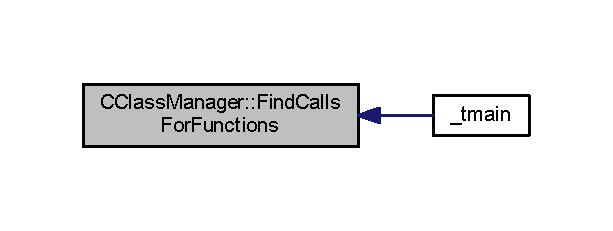
\includegraphics[width=294pt]{class_c_class_manager_a7a44afac10c69c87860c65040b23b57a_icgraph}
\end{center}
\end{figure}


\hypertarget{class_c_class_manager_a1db9b102548bc1b9becf44031d5c3937}{\index{C\+Class\+Manager@{C\+Class\+Manager}!Find\+Class@{Find\+Class}}
\index{Find\+Class@{Find\+Class}!C\+Class\+Manager@{C\+Class\+Manager}}
\subsubsection[{Find\+Class}]{\setlength{\rightskip}{0pt plus 5cm}bool C\+Class\+Manager\+::\+Find\+Class (
\begin{DoxyParamCaption}
\item[{string}]{a\+\_\+sz\+Files\+Path}
\end{DoxyParamCaption}
)\hspace{0.3cm}{\ttfamily [private]}}}\label{class_c_class_manager_a1db9b102548bc1b9becf44031d5c3937}


Here is the caller graph for this function\+:
\nopagebreak
\begin{figure}[H]
\begin{center}
\leavevmode
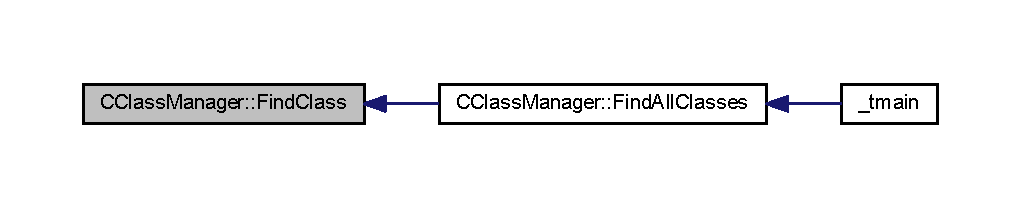
\includegraphics[width=350pt]{class_c_class_manager_a1db9b102548bc1b9becf44031d5c3937_icgraph}
\end{center}
\end{figure}


\hypertarget{class_c_class_manager_a1df8fae08901fc20f20e7f7f5120d267}{\index{C\+Class\+Manager@{C\+Class\+Manager}!Find\+Functions@{Find\+Functions}}
\index{Find\+Functions@{Find\+Functions}!C\+Class\+Manager@{C\+Class\+Manager}}
\subsubsection[{Find\+Functions}]{\setlength{\rightskip}{0pt plus 5cm}bool C\+Class\+Manager\+::\+Find\+Functions (
\begin{DoxyParamCaption}
{}
\end{DoxyParamCaption}
)}}\label{class_c_class_manager_a1df8fae08901fc20f20e7f7f5120d267}


Here is the caller graph for this function\+:
\nopagebreak
\begin{figure}[H]
\begin{center}
\leavevmode
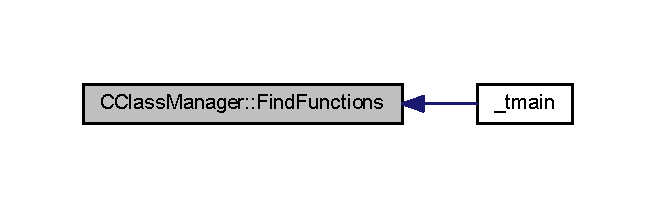
\includegraphics[width=315pt]{class_c_class_manager_a1df8fae08901fc20f20e7f7f5120d267_icgraph}
\end{center}
\end{figure}


\hypertarget{class_c_class_manager_a7a5bd390df1b4100f452d56f94cadf24}{\index{C\+Class\+Manager@{C\+Class\+Manager}!Show\+All\+Classes@{Show\+All\+Classes}}
\index{Show\+All\+Classes@{Show\+All\+Classes}!C\+Class\+Manager@{C\+Class\+Manager}}
\subsubsection[{Show\+All\+Classes}]{\setlength{\rightskip}{0pt plus 5cm}void C\+Class\+Manager\+::\+Show\+All\+Classes (
\begin{DoxyParamCaption}
{}
\end{DoxyParamCaption}
)}}\label{class_c_class_manager_a7a5bd390df1b4100f452d56f94cadf24}


\subsection{Member Data Documentation}
\hypertarget{class_c_class_manager_a6ea255cab18dff35dd07390af7776675}{\index{C\+Class\+Manager@{C\+Class\+Manager}!m\+\_\+p\+Files\+Finder@{m\+\_\+p\+Files\+Finder}}
\index{m\+\_\+p\+Files\+Finder@{m\+\_\+p\+Files\+Finder}!C\+Class\+Manager@{C\+Class\+Manager}}
\subsubsection[{m\+\_\+p\+Files\+Finder}]{\setlength{\rightskip}{0pt plus 5cm}{\bf C\+Files\+Finder}$\ast$ C\+Class\+Manager\+::m\+\_\+p\+Files\+Finder\hspace{0.3cm}{\ttfamily [private]}}}\label{class_c_class_manager_a6ea255cab18dff35dd07390af7776675}
\hypertarget{class_c_class_manager_acbcada64d77a7fa05c8c6ffadcf730db}{\index{C\+Class\+Manager@{C\+Class\+Manager}!m\+\_\+sz\+Classes\+List@{m\+\_\+sz\+Classes\+List}}
\index{m\+\_\+sz\+Classes\+List@{m\+\_\+sz\+Classes\+List}!C\+Class\+Manager@{C\+Class\+Manager}}
\subsubsection[{m\+\_\+sz\+Classes\+List}]{\setlength{\rightskip}{0pt plus 5cm}std\+::vector$<${\bf C\+Class}$>$ C\+Class\+Manager\+::m\+\_\+sz\+Classes\+List\hspace{0.3cm}{\ttfamily [protected]}}}\label{class_c_class_manager_acbcada64d77a7fa05c8c6ffadcf730db}


The documentation for this class was generated from the following files\+:\begin{DoxyCompactItemize}
\item 
diagrams/\hyperlink{_class_manager_8h}{Class\+Manager.\+h}\item 
diagrams/\hyperlink{_class_manager_8cpp}{Class\+Manager.\+cpp}\end{DoxyCompactItemize}

\hypertarget{class_c_files_finder}{\section{C\+Files\+Finder Class Reference}
\label{class_c_files_finder}\index{C\+Files\+Finder@{C\+Files\+Finder}}
}


{\ttfamily \#include $<$Files\+Finder.\+h$>$}



Collaboration diagram for C\+Files\+Finder\+:
\nopagebreak
\begin{figure}[H]
\begin{center}
\leavevmode
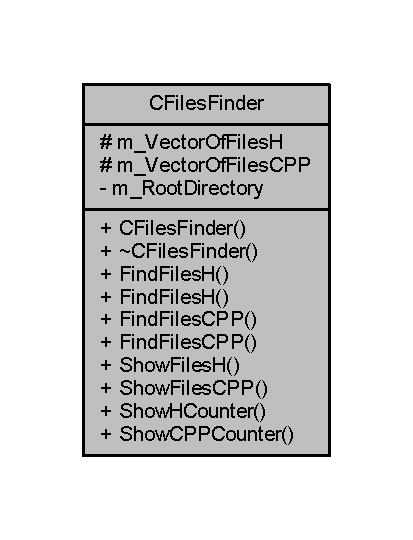
\includegraphics[width=198pt]{class_c_files_finder__coll__graph}
\end{center}
\end{figure}
\subsection*{Classes}
\begin{DoxyCompactItemize}
\item 
struct \hyperlink{struct_c_files_finder_1_1_s_file}{S\+File}
\end{DoxyCompactItemize}
\subsection*{Public Member Functions}
\begin{DoxyCompactItemize}
\item 
\hyperlink{class_c_files_finder_a2d82e60f3f4a90fa03d680ad0801abea}{C\+Files\+Finder} (string a\+\_\+\+Root\+Directory)
\item 
\hyperlink{class_c_files_finder_aa35e985107f5cb7997a31d787de31aba}{$\sim$\+C\+Files\+Finder} ()
\item 
bool \hyperlink{class_c_files_finder_a1a904fd47c4d9a1766cb18562a9e083b}{Find\+Files\+H} ()
\item 
bool \hyperlink{class_c_files_finder_abf39e6926090d2d0494b5ca18d40617f}{Find\+Files\+H} (string a\+\_\+\+Root\+Directory)
\item 
bool \hyperlink{class_c_files_finder_a6669f0338caec55ef9d4407fffd4440f}{Find\+Files\+C\+P\+P} ()
\item 
bool \hyperlink{class_c_files_finder_aa18e8c325b9da120f55d0091f802e95c}{Find\+Files\+C\+P\+P} (string a\+\_\+\+Root\+Directory)
\item 
void \hyperlink{class_c_files_finder_ae391c3d03d56c7f9af84ad2a52085365}{Show\+Files\+H} ()
\item 
void \hyperlink{class_c_files_finder_a4c7cc8eab39706cd8dc9c73e186f98f7}{Show\+Files\+C\+P\+P} ()
\item 
void \hyperlink{class_c_files_finder_a0aee1050295a066330dc0f2974089006}{Show\+H\+Counter} ()
\item 
void \hyperlink{class_c_files_finder_a7929f2dcfcd7bef8e1530e999eb05a4d}{Show\+C\+P\+P\+Counter} ()
\end{DoxyCompactItemize}
\subsection*{Protected Attributes}
\begin{DoxyCompactItemize}
\item 
vector$<$ \hyperlink{struct_c_files_finder_1_1_s_file}{S\+File} $>$ \hyperlink{class_c_files_finder_a2a737438eb2515c0d494b0d4edca3808}{m\+\_\+\+Vector\+Of\+Files\+H}
\item 
vector$<$ \hyperlink{struct_c_files_finder_1_1_s_file}{S\+File} $>$ \hyperlink{class_c_files_finder_a2c6b3e50076b2a5e84a872982fd74f8e}{m\+\_\+\+Vector\+Of\+Files\+C\+P\+P}
\end{DoxyCompactItemize}
\subsection*{Private Attributes}
\begin{DoxyCompactItemize}
\item 
string \hyperlink{class_c_files_finder_a4ed42fa95872f6c774ce1b1672877f96}{m\+\_\+\+Root\+Directory}
\end{DoxyCompactItemize}
\subsection*{Friends}
\begin{DoxyCompactItemize}
\item 
class \hyperlink{class_c_files_finder_a160d67be17e37e9f9a8ca10aa20e8ff1}{C\+Class\+Manager}
\item 
class \hyperlink{class_c_files_finder_ae2f76f286ff7f2c3836026f880f0438e}{C\+Class}
\end{DoxyCompactItemize}


\subsection{Constructor \& Destructor Documentation}
\hypertarget{class_c_files_finder_a2d82e60f3f4a90fa03d680ad0801abea}{\index{C\+Files\+Finder@{C\+Files\+Finder}!C\+Files\+Finder@{C\+Files\+Finder}}
\index{C\+Files\+Finder@{C\+Files\+Finder}!C\+Files\+Finder@{C\+Files\+Finder}}
\subsubsection[{C\+Files\+Finder}]{\setlength{\rightskip}{0pt plus 5cm}C\+Files\+Finder\+::\+C\+Files\+Finder (
\begin{DoxyParamCaption}
\item[{string}]{a\+\_\+\+Root\+Directory}
\end{DoxyParamCaption}
)}}\label{class_c_files_finder_a2d82e60f3f4a90fa03d680ad0801abea}
\hypertarget{class_c_files_finder_aa35e985107f5cb7997a31d787de31aba}{\index{C\+Files\+Finder@{C\+Files\+Finder}!````~C\+Files\+Finder@{$\sim$\+C\+Files\+Finder}}
\index{````~C\+Files\+Finder@{$\sim$\+C\+Files\+Finder}!C\+Files\+Finder@{C\+Files\+Finder}}
\subsubsection[{$\sim$\+C\+Files\+Finder}]{\setlength{\rightskip}{0pt plus 5cm}C\+Files\+Finder\+::$\sim$\+C\+Files\+Finder (
\begin{DoxyParamCaption}
{}
\end{DoxyParamCaption}
)}}\label{class_c_files_finder_aa35e985107f5cb7997a31d787de31aba}


\subsection{Member Function Documentation}
\hypertarget{class_c_files_finder_a6669f0338caec55ef9d4407fffd4440f}{\index{C\+Files\+Finder@{C\+Files\+Finder}!Find\+Files\+C\+P\+P@{Find\+Files\+C\+P\+P}}
\index{Find\+Files\+C\+P\+P@{Find\+Files\+C\+P\+P}!C\+Files\+Finder@{C\+Files\+Finder}}
\subsubsection[{Find\+Files\+C\+P\+P}]{\setlength{\rightskip}{0pt plus 5cm}bool C\+Files\+Finder\+::\+Find\+Files\+C\+P\+P (
\begin{DoxyParamCaption}
{}
\end{DoxyParamCaption}
)}}\label{class_c_files_finder_a6669f0338caec55ef9d4407fffd4440f}


Here is the caller graph for this function\+:
\nopagebreak
\begin{figure}[H]
\begin{center}
\leavevmode
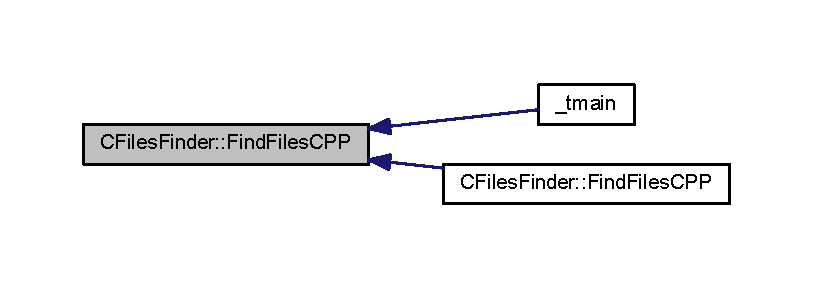
\includegraphics[width=350pt]{class_c_files_finder_a6669f0338caec55ef9d4407fffd4440f_icgraph}
\end{center}
\end{figure}


\hypertarget{class_c_files_finder_aa18e8c325b9da120f55d0091f802e95c}{\index{C\+Files\+Finder@{C\+Files\+Finder}!Find\+Files\+C\+P\+P@{Find\+Files\+C\+P\+P}}
\index{Find\+Files\+C\+P\+P@{Find\+Files\+C\+P\+P}!C\+Files\+Finder@{C\+Files\+Finder}}
\subsubsection[{Find\+Files\+C\+P\+P}]{\setlength{\rightskip}{0pt plus 5cm}bool C\+Files\+Finder\+::\+Find\+Files\+C\+P\+P (
\begin{DoxyParamCaption}
\item[{string}]{a\+\_\+\+Root\+Directory}
\end{DoxyParamCaption}
)}}\label{class_c_files_finder_aa18e8c325b9da120f55d0091f802e95c}


Here is the call graph for this function\+:
\nopagebreak
\begin{figure}[H]
\begin{center}
\leavevmode
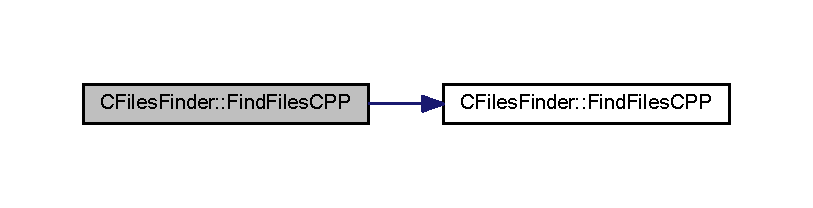
\includegraphics[width=350pt]{class_c_files_finder_aa18e8c325b9da120f55d0091f802e95c_cgraph}
\end{center}
\end{figure}


\hypertarget{class_c_files_finder_a1a904fd47c4d9a1766cb18562a9e083b}{\index{C\+Files\+Finder@{C\+Files\+Finder}!Find\+Files\+H@{Find\+Files\+H}}
\index{Find\+Files\+H@{Find\+Files\+H}!C\+Files\+Finder@{C\+Files\+Finder}}
\subsubsection[{Find\+Files\+H}]{\setlength{\rightskip}{0pt plus 5cm}bool C\+Files\+Finder\+::\+Find\+Files\+H (
\begin{DoxyParamCaption}
{}
\end{DoxyParamCaption}
)}}\label{class_c_files_finder_a1a904fd47c4d9a1766cb18562a9e083b}


Here is the caller graph for this function\+:
\nopagebreak
\begin{figure}[H]
\begin{center}
\leavevmode
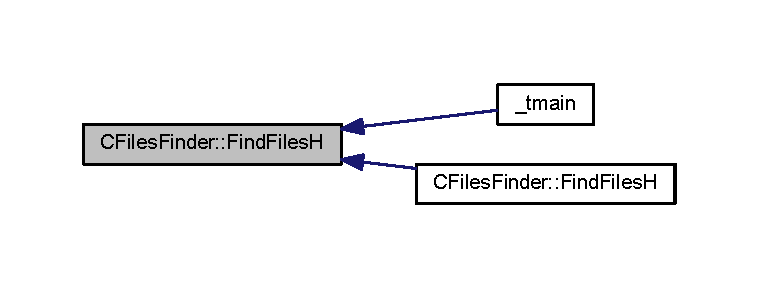
\includegraphics[width=350pt]{class_c_files_finder_a1a904fd47c4d9a1766cb18562a9e083b_icgraph}
\end{center}
\end{figure}


\hypertarget{class_c_files_finder_abf39e6926090d2d0494b5ca18d40617f}{\index{C\+Files\+Finder@{C\+Files\+Finder}!Find\+Files\+H@{Find\+Files\+H}}
\index{Find\+Files\+H@{Find\+Files\+H}!C\+Files\+Finder@{C\+Files\+Finder}}
\subsubsection[{Find\+Files\+H}]{\setlength{\rightskip}{0pt plus 5cm}bool C\+Files\+Finder\+::\+Find\+Files\+H (
\begin{DoxyParamCaption}
\item[{string}]{a\+\_\+\+Root\+Directory}
\end{DoxyParamCaption}
)}}\label{class_c_files_finder_abf39e6926090d2d0494b5ca18d40617f}


Here is the call graph for this function\+:
\nopagebreak
\begin{figure}[H]
\begin{center}
\leavevmode
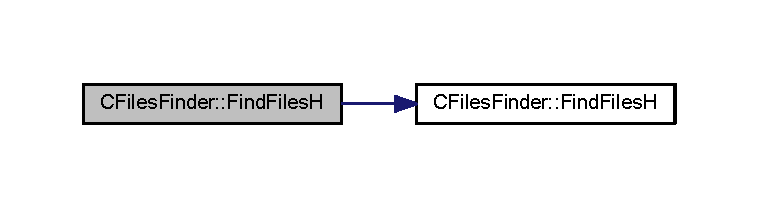
\includegraphics[width=350pt]{class_c_files_finder_abf39e6926090d2d0494b5ca18d40617f_cgraph}
\end{center}
\end{figure}


\hypertarget{class_c_files_finder_a7929f2dcfcd7bef8e1530e999eb05a4d}{\index{C\+Files\+Finder@{C\+Files\+Finder}!Show\+C\+P\+P\+Counter@{Show\+C\+P\+P\+Counter}}
\index{Show\+C\+P\+P\+Counter@{Show\+C\+P\+P\+Counter}!C\+Files\+Finder@{C\+Files\+Finder}}
\subsubsection[{Show\+C\+P\+P\+Counter}]{\setlength{\rightskip}{0pt plus 5cm}void C\+Files\+Finder\+::\+Show\+C\+P\+P\+Counter (
\begin{DoxyParamCaption}
{}
\end{DoxyParamCaption}
)}}\label{class_c_files_finder_a7929f2dcfcd7bef8e1530e999eb05a4d}


Here is the caller graph for this function\+:
\nopagebreak
\begin{figure}[H]
\begin{center}
\leavevmode
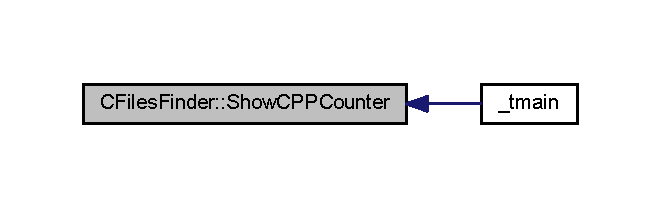
\includegraphics[width=317pt]{class_c_files_finder_a7929f2dcfcd7bef8e1530e999eb05a4d_icgraph}
\end{center}
\end{figure}


\hypertarget{class_c_files_finder_a4c7cc8eab39706cd8dc9c73e186f98f7}{\index{C\+Files\+Finder@{C\+Files\+Finder}!Show\+Files\+C\+P\+P@{Show\+Files\+C\+P\+P}}
\index{Show\+Files\+C\+P\+P@{Show\+Files\+C\+P\+P}!C\+Files\+Finder@{C\+Files\+Finder}}
\subsubsection[{Show\+Files\+C\+P\+P}]{\setlength{\rightskip}{0pt plus 5cm}void C\+Files\+Finder\+::\+Show\+Files\+C\+P\+P (
\begin{DoxyParamCaption}
{}
\end{DoxyParamCaption}
)}}\label{class_c_files_finder_a4c7cc8eab39706cd8dc9c73e186f98f7}
\hypertarget{class_c_files_finder_ae391c3d03d56c7f9af84ad2a52085365}{\index{C\+Files\+Finder@{C\+Files\+Finder}!Show\+Files\+H@{Show\+Files\+H}}
\index{Show\+Files\+H@{Show\+Files\+H}!C\+Files\+Finder@{C\+Files\+Finder}}
\subsubsection[{Show\+Files\+H}]{\setlength{\rightskip}{0pt plus 5cm}void C\+Files\+Finder\+::\+Show\+Files\+H (
\begin{DoxyParamCaption}
{}
\end{DoxyParamCaption}
)}}\label{class_c_files_finder_ae391c3d03d56c7f9af84ad2a52085365}
\hypertarget{class_c_files_finder_a0aee1050295a066330dc0f2974089006}{\index{C\+Files\+Finder@{C\+Files\+Finder}!Show\+H\+Counter@{Show\+H\+Counter}}
\index{Show\+H\+Counter@{Show\+H\+Counter}!C\+Files\+Finder@{C\+Files\+Finder}}
\subsubsection[{Show\+H\+Counter}]{\setlength{\rightskip}{0pt plus 5cm}void C\+Files\+Finder\+::\+Show\+H\+Counter (
\begin{DoxyParamCaption}
{}
\end{DoxyParamCaption}
)}}\label{class_c_files_finder_a0aee1050295a066330dc0f2974089006}


Here is the caller graph for this function\+:
\nopagebreak
\begin{figure}[H]
\begin{center}
\leavevmode
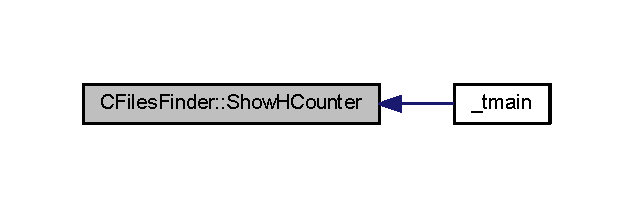
\includegraphics[width=304pt]{class_c_files_finder_a0aee1050295a066330dc0f2974089006_icgraph}
\end{center}
\end{figure}




\subsection{Friends And Related Function Documentation}
\hypertarget{class_c_files_finder_ae2f76f286ff7f2c3836026f880f0438e}{\index{C\+Files\+Finder@{C\+Files\+Finder}!C\+Class@{C\+Class}}
\index{C\+Class@{C\+Class}!C\+Files\+Finder@{C\+Files\+Finder}}
\subsubsection[{C\+Class}]{\setlength{\rightskip}{0pt plus 5cm}friend class {\bf C\+Class}\hspace{0.3cm}{\ttfamily [friend]}}}\label{class_c_files_finder_ae2f76f286ff7f2c3836026f880f0438e}
\hypertarget{class_c_files_finder_a160d67be17e37e9f9a8ca10aa20e8ff1}{\index{C\+Files\+Finder@{C\+Files\+Finder}!C\+Class\+Manager@{C\+Class\+Manager}}
\index{C\+Class\+Manager@{C\+Class\+Manager}!C\+Files\+Finder@{C\+Files\+Finder}}
\subsubsection[{C\+Class\+Manager}]{\setlength{\rightskip}{0pt plus 5cm}friend class {\bf C\+Class\+Manager}\hspace{0.3cm}{\ttfamily [friend]}}}\label{class_c_files_finder_a160d67be17e37e9f9a8ca10aa20e8ff1}


\subsection{Member Data Documentation}
\hypertarget{class_c_files_finder_a4ed42fa95872f6c774ce1b1672877f96}{\index{C\+Files\+Finder@{C\+Files\+Finder}!m\+\_\+\+Root\+Directory@{m\+\_\+\+Root\+Directory}}
\index{m\+\_\+\+Root\+Directory@{m\+\_\+\+Root\+Directory}!C\+Files\+Finder@{C\+Files\+Finder}}
\subsubsection[{m\+\_\+\+Root\+Directory}]{\setlength{\rightskip}{0pt plus 5cm}string C\+Files\+Finder\+::m\+\_\+\+Root\+Directory\hspace{0.3cm}{\ttfamily [private]}}}\label{class_c_files_finder_a4ed42fa95872f6c774ce1b1672877f96}
\hypertarget{class_c_files_finder_a2c6b3e50076b2a5e84a872982fd74f8e}{\index{C\+Files\+Finder@{C\+Files\+Finder}!m\+\_\+\+Vector\+Of\+Files\+C\+P\+P@{m\+\_\+\+Vector\+Of\+Files\+C\+P\+P}}
\index{m\+\_\+\+Vector\+Of\+Files\+C\+P\+P@{m\+\_\+\+Vector\+Of\+Files\+C\+P\+P}!C\+Files\+Finder@{C\+Files\+Finder}}
\subsubsection[{m\+\_\+\+Vector\+Of\+Files\+C\+P\+P}]{\setlength{\rightskip}{0pt plus 5cm}vector$<${\bf S\+File}$>$ C\+Files\+Finder\+::m\+\_\+\+Vector\+Of\+Files\+C\+P\+P\hspace{0.3cm}{\ttfamily [protected]}}}\label{class_c_files_finder_a2c6b3e50076b2a5e84a872982fd74f8e}
\hypertarget{class_c_files_finder_a2a737438eb2515c0d494b0d4edca3808}{\index{C\+Files\+Finder@{C\+Files\+Finder}!m\+\_\+\+Vector\+Of\+Files\+H@{m\+\_\+\+Vector\+Of\+Files\+H}}
\index{m\+\_\+\+Vector\+Of\+Files\+H@{m\+\_\+\+Vector\+Of\+Files\+H}!C\+Files\+Finder@{C\+Files\+Finder}}
\subsubsection[{m\+\_\+\+Vector\+Of\+Files\+H}]{\setlength{\rightskip}{0pt plus 5cm}vector$<${\bf S\+File}$>$ C\+Files\+Finder\+::m\+\_\+\+Vector\+Of\+Files\+H\hspace{0.3cm}{\ttfamily [protected]}}}\label{class_c_files_finder_a2a737438eb2515c0d494b0d4edca3808}


The documentation for this class was generated from the following files\+:\begin{DoxyCompactItemize}
\item 
diagrams/\hyperlink{_files_finder_8h}{Files\+Finder.\+h}\item 
diagrams/\hyperlink{_files_finder_8cpp}{Files\+Finder.\+cpp}\end{DoxyCompactItemize}

\hypertarget{struct_c_files_finder_1_1_s_file}{\section{C\+Files\+Finder\+:\+:S\+File Struct Reference}
\label{struct_c_files_finder_1_1_s_file}\index{C\+Files\+Finder\+::\+S\+File@{C\+Files\+Finder\+::\+S\+File}}
}


Collaboration diagram for C\+Files\+Finder\+:\+:S\+File\+:
\nopagebreak
\begin{figure}[H]
\begin{center}
\leavevmode
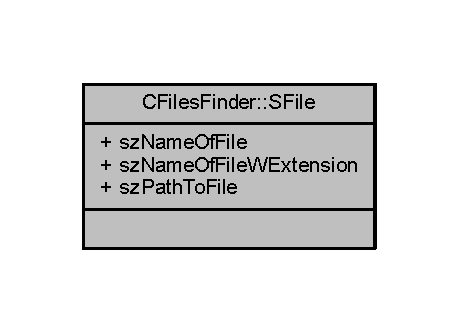
\includegraphics[width=220pt]{struct_c_files_finder_1_1_s_file__coll__graph}
\end{center}
\end{figure}
\subsection*{Public Attributes}
\begin{DoxyCompactItemize}
\item 
string \hyperlink{struct_c_files_finder_1_1_s_file_aaed5de486dfbdb594746e4fd13c65074}{sz\+Name\+Of\+File}
\item 
string \hyperlink{struct_c_files_finder_1_1_s_file_a7ceceb85e185f30be5476a3d150a2aba}{sz\+Name\+Of\+File\+W\+Extension}
\item 
string \hyperlink{struct_c_files_finder_1_1_s_file_aa0ec885df98370ebdd2fdb429ce76adf}{sz\+Path\+To\+File}
\end{DoxyCompactItemize}


\subsection{Member Data Documentation}
\hypertarget{struct_c_files_finder_1_1_s_file_aaed5de486dfbdb594746e4fd13c65074}{\index{C\+Files\+Finder\+::\+S\+File@{C\+Files\+Finder\+::\+S\+File}!sz\+Name\+Of\+File@{sz\+Name\+Of\+File}}
\index{sz\+Name\+Of\+File@{sz\+Name\+Of\+File}!C\+Files\+Finder\+::\+S\+File@{C\+Files\+Finder\+::\+S\+File}}
\subsubsection[{sz\+Name\+Of\+File}]{\setlength{\rightskip}{0pt plus 5cm}string C\+Files\+Finder\+::\+S\+File\+::sz\+Name\+Of\+File}}\label{struct_c_files_finder_1_1_s_file_aaed5de486dfbdb594746e4fd13c65074}
\hypertarget{struct_c_files_finder_1_1_s_file_a7ceceb85e185f30be5476a3d150a2aba}{\index{C\+Files\+Finder\+::\+S\+File@{C\+Files\+Finder\+::\+S\+File}!sz\+Name\+Of\+File\+W\+Extension@{sz\+Name\+Of\+File\+W\+Extension}}
\index{sz\+Name\+Of\+File\+W\+Extension@{sz\+Name\+Of\+File\+W\+Extension}!C\+Files\+Finder\+::\+S\+File@{C\+Files\+Finder\+::\+S\+File}}
\subsubsection[{sz\+Name\+Of\+File\+W\+Extension}]{\setlength{\rightskip}{0pt plus 5cm}string C\+Files\+Finder\+::\+S\+File\+::sz\+Name\+Of\+File\+W\+Extension}}\label{struct_c_files_finder_1_1_s_file_a7ceceb85e185f30be5476a3d150a2aba}
\hypertarget{struct_c_files_finder_1_1_s_file_aa0ec885df98370ebdd2fdb429ce76adf}{\index{C\+Files\+Finder\+::\+S\+File@{C\+Files\+Finder\+::\+S\+File}!sz\+Path\+To\+File@{sz\+Path\+To\+File}}
\index{sz\+Path\+To\+File@{sz\+Path\+To\+File}!C\+Files\+Finder\+::\+S\+File@{C\+Files\+Finder\+::\+S\+File}}
\subsubsection[{sz\+Path\+To\+File}]{\setlength{\rightskip}{0pt plus 5cm}string C\+Files\+Finder\+::\+S\+File\+::sz\+Path\+To\+File}}\label{struct_c_files_finder_1_1_s_file_aa0ec885df98370ebdd2fdb429ce76adf}


The documentation for this struct was generated from the following file\+:\begin{DoxyCompactItemize}
\item 
diagrams/\hyperlink{_files_finder_8h}{Files\+Finder.\+h}\end{DoxyCompactItemize}

\hypertarget{struct_c_class_1_1_s_function}{\section{C\+Class\+:\+:S\+Function Struct Reference}
\label{struct_c_class_1_1_s_function}\index{C\+Class\+::\+S\+Function@{C\+Class\+::\+S\+Function}}
}


{\ttfamily \#include $<$Class.\+h$>$}



Collaboration diagram for C\+Class\+:\+:S\+Function\+:
\nopagebreak
\begin{figure}[H]
\begin{center}
\leavevmode
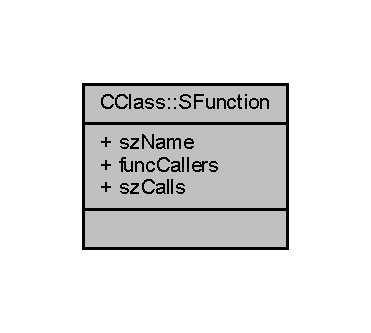
\includegraphics[width=178pt]{struct_c_class_1_1_s_function__coll__graph}
\end{center}
\end{figure}
\subsection*{Public Attributes}
\begin{DoxyCompactItemize}
\item 
string \hyperlink{struct_c_class_1_1_s_function_a709a1e1916aa5921620198effa41c8b5}{sz\+Name}
\item 
vector$<$ \hyperlink{struct_c_class_1_1_s_function}{S\+Function} $>$ \hyperlink{struct_c_class_1_1_s_function_a7ac14ba0820fd54ae22e34f2e88fe2e9}{func\+Callers}
\item 
vector$<$ string $>$ \hyperlink{struct_c_class_1_1_s_function_a389c0be3f14b06b53b919ba6e4eb7063}{sz\+Calls}
\end{DoxyCompactItemize}


\subsection{Member Data Documentation}
\hypertarget{struct_c_class_1_1_s_function_a7ac14ba0820fd54ae22e34f2e88fe2e9}{\index{C\+Class\+::\+S\+Function@{C\+Class\+::\+S\+Function}!func\+Callers@{func\+Callers}}
\index{func\+Callers@{func\+Callers}!C\+Class\+::\+S\+Function@{C\+Class\+::\+S\+Function}}
\subsubsection[{func\+Callers}]{\setlength{\rightskip}{0pt plus 5cm}vector$<${\bf S\+Function}$>$ C\+Class\+::\+S\+Function\+::func\+Callers}}\label{struct_c_class_1_1_s_function_a7ac14ba0820fd54ae22e34f2e88fe2e9}
\hypertarget{struct_c_class_1_1_s_function_a389c0be3f14b06b53b919ba6e4eb7063}{\index{C\+Class\+::\+S\+Function@{C\+Class\+::\+S\+Function}!sz\+Calls@{sz\+Calls}}
\index{sz\+Calls@{sz\+Calls}!C\+Class\+::\+S\+Function@{C\+Class\+::\+S\+Function}}
\subsubsection[{sz\+Calls}]{\setlength{\rightskip}{0pt plus 5cm}vector$<$string$>$ C\+Class\+::\+S\+Function\+::sz\+Calls}}\label{struct_c_class_1_1_s_function_a389c0be3f14b06b53b919ba6e4eb7063}
\hypertarget{struct_c_class_1_1_s_function_a709a1e1916aa5921620198effa41c8b5}{\index{C\+Class\+::\+S\+Function@{C\+Class\+::\+S\+Function}!sz\+Name@{sz\+Name}}
\index{sz\+Name@{sz\+Name}!C\+Class\+::\+S\+Function@{C\+Class\+::\+S\+Function}}
\subsubsection[{sz\+Name}]{\setlength{\rightskip}{0pt plus 5cm}string C\+Class\+::\+S\+Function\+::sz\+Name}}\label{struct_c_class_1_1_s_function_a709a1e1916aa5921620198effa41c8b5}


The documentation for this struct was generated from the following file\+:\begin{DoxyCompactItemize}
\item 
diagrams/\hyperlink{_class_8h}{Class.\+h}\end{DoxyCompactItemize}

\chapter{File Documentation}
\hypertarget{_class_8cpp}{\section{diagrams/\+Class.cpp File Reference}
\label{_class_8cpp}\index{diagrams/\+Class.\+cpp@{diagrams/\+Class.\+cpp}}
}
{\ttfamily \#include \char`\"{}stdafx.\+h\char`\"{}}\\*
{\ttfamily \#include \char`\"{}Class.\+h\char`\"{}}\\*
{\ttfamily \#include $<$iostream$>$}\\*
{\ttfamily \#include $<$fstream$>$}\\*
{\ttfamily \#include $<$string$>$}\\*
{\ttfamily \#include $<$regex$>$}\\*
{\ttfamily \#include $<$windows.\+h$>$}\\*
Include dependency graph for Class.\+cpp\+:
\nopagebreak
\begin{figure}[H]
\begin{center}
\leavevmode
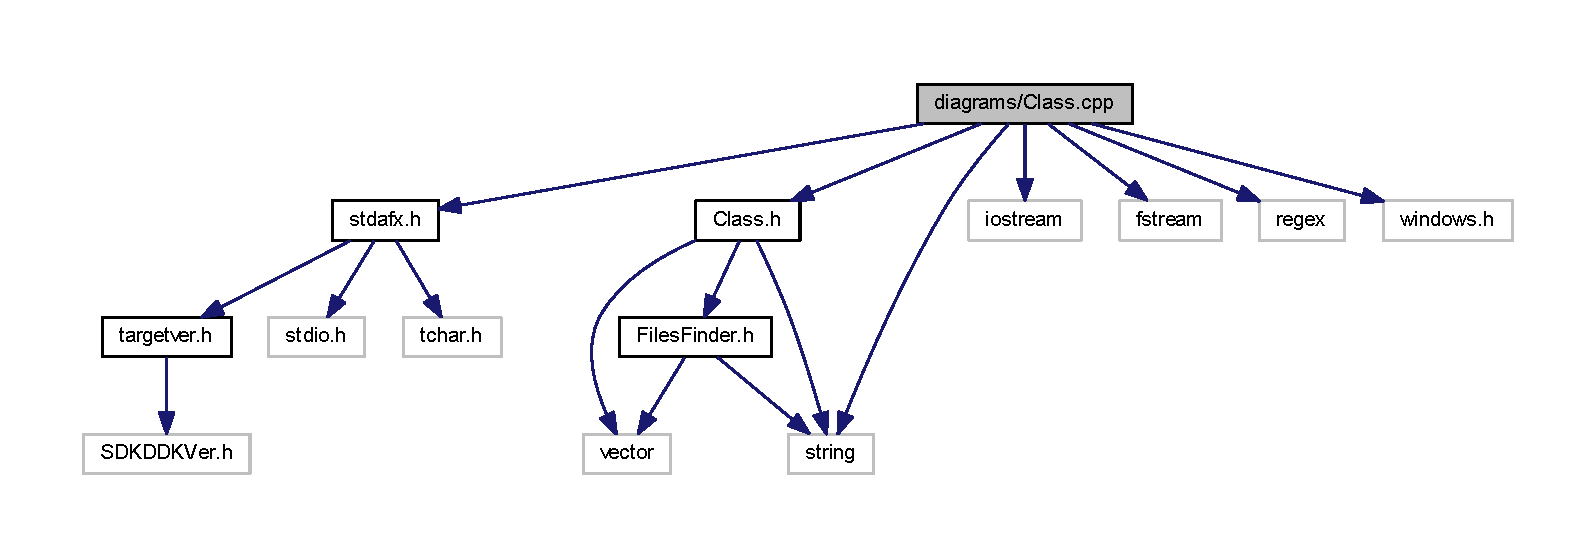
\includegraphics[width=350pt]{_class_8cpp__incl}
\end{center}
\end{figure}

\hypertarget{_class_8h}{\section{diagrams/\+Class.h File Reference}
\label{_class_8h}\index{diagrams/\+Class.\+h@{diagrams/\+Class.\+h}}
}
{\ttfamily \#include $<$vector$>$}\\*
{\ttfamily \#include $<$string$>$}\\*
{\ttfamily \#include \char`\"{}Files\+Finder.\+h\char`\"{}}\\*
Include dependency graph for Class.\+h\+:
\nopagebreak
\begin{figure}[H]
\begin{center}
\leavevmode
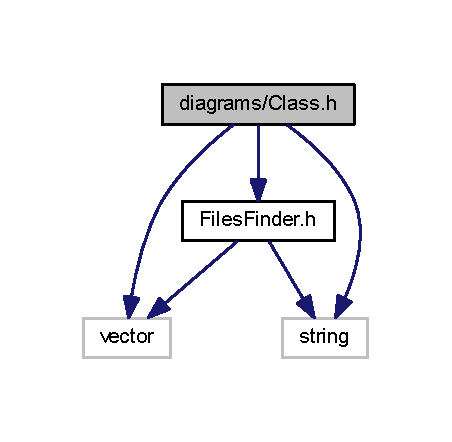
\includegraphics[width=217pt]{_class_8h__incl}
\end{center}
\end{figure}
This graph shows which files directly or indirectly include this file\+:
\nopagebreak
\begin{figure}[H]
\begin{center}
\leavevmode
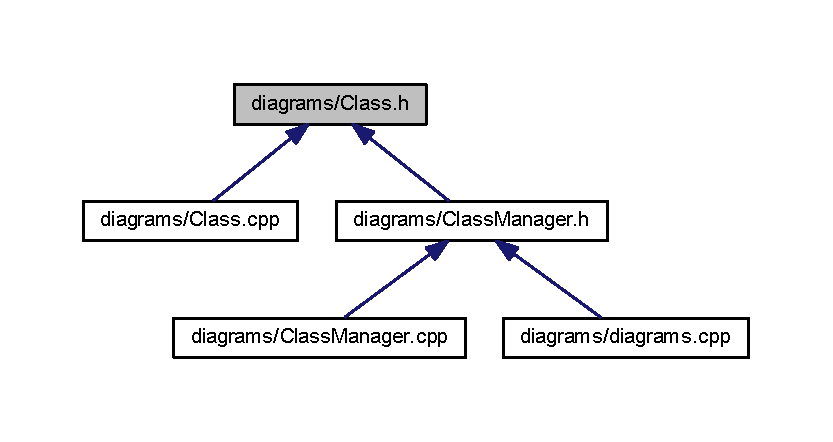
\includegraphics[width=350pt]{_class_8h__dep__incl}
\end{center}
\end{figure}
\subsection*{Classes}
\begin{DoxyCompactItemize}
\item 
class \hyperlink{class_c_class}{C\+Class}
\item 
struct \hyperlink{struct_c_class_1_1_s_function}{C\+Class\+::\+S\+Function}
\end{DoxyCompactItemize}

\hypertarget{_class_manager_8cpp}{\section{diagrams/\+Class\+Manager.cpp File Reference}
\label{_class_manager_8cpp}\index{diagrams/\+Class\+Manager.\+cpp@{diagrams/\+Class\+Manager.\+cpp}}
}
{\ttfamily \#include \char`\"{}stdafx.\+h\char`\"{}}\\*
{\ttfamily \#include \char`\"{}Class\+Manager.\+h\char`\"{}}\\*
{\ttfamily \#include $<$iostream$>$}\\*
{\ttfamily \#include $<$fstream$>$}\\*
{\ttfamily \#include $<$string$>$}\\*
{\ttfamily \#include $<$regex$>$}\\*
Include dependency graph for Class\+Manager.\+cpp\+:
\nopagebreak
\begin{figure}[H]
\begin{center}
\leavevmode
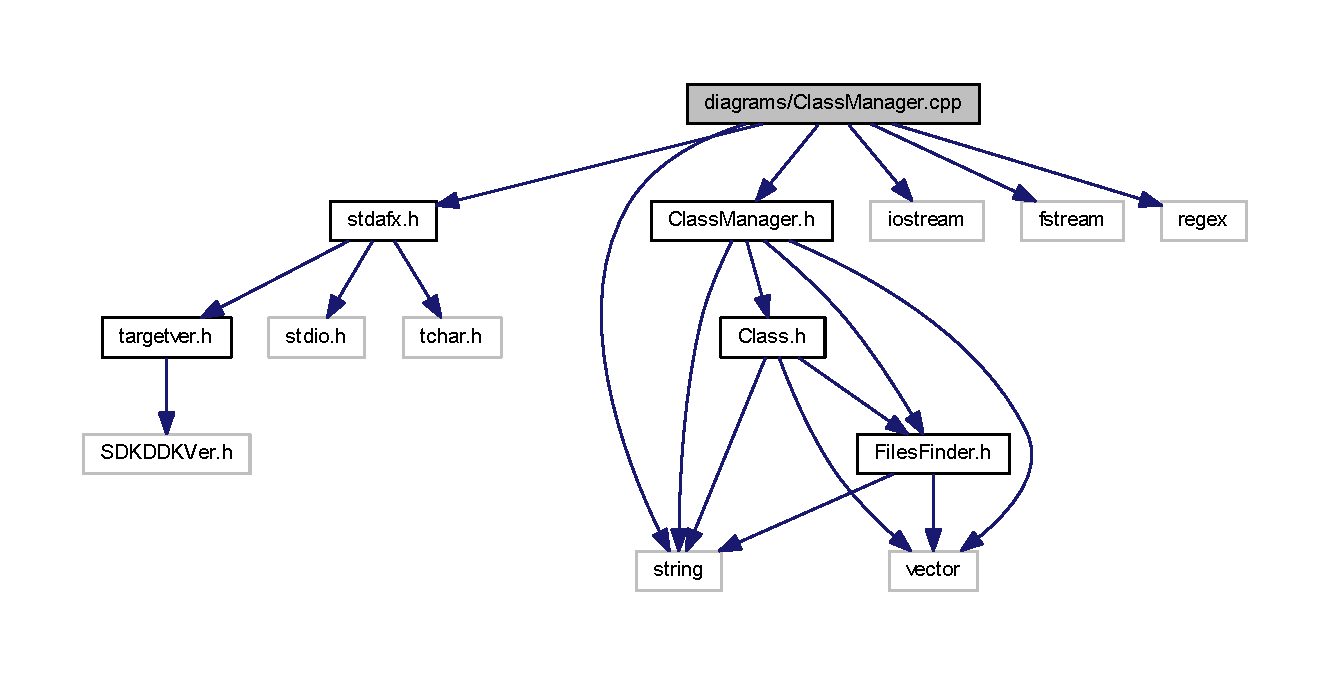
\includegraphics[width=350pt]{_class_manager_8cpp__incl}
\end{center}
\end{figure}

\hypertarget{_class_manager_8h}{\section{diagrams/\+Class\+Manager.h File Reference}
\label{_class_manager_8h}\index{diagrams/\+Class\+Manager.\+h@{diagrams/\+Class\+Manager.\+h}}
}
{\ttfamily \#include \char`\"{}Files\+Finder.\+h\char`\"{}}\\*
{\ttfamily \#include \char`\"{}Class.\+h\char`\"{}}\\*
{\ttfamily \#include $<$vector$>$}\\*
{\ttfamily \#include $<$string$>$}\\*
Include dependency graph for Class\+Manager.\+h\+:
\nopagebreak
\begin{figure}[H]
\begin{center}
\leavevmode
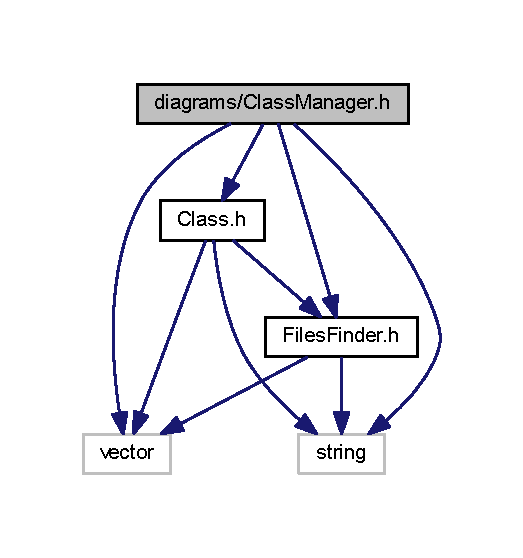
\includegraphics[width=251pt]{_class_manager_8h__incl}
\end{center}
\end{figure}
This graph shows which files directly or indirectly include this file\+:
\nopagebreak
\begin{figure}[H]
\begin{center}
\leavevmode
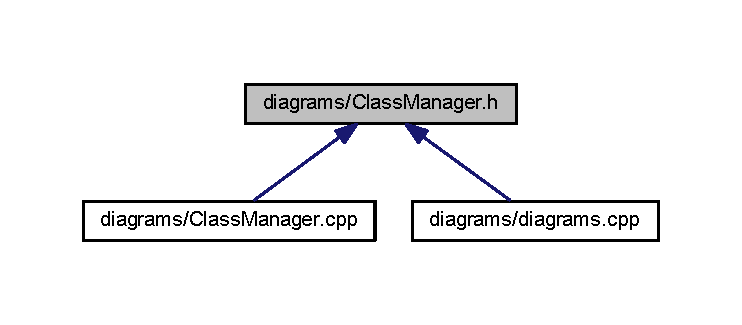
\includegraphics[width=350pt]{_class_manager_8h__dep__incl}
\end{center}
\end{figure}
\subsection*{Classes}
\begin{DoxyCompactItemize}
\item 
class \hyperlink{class_c_class_manager}{C\+Class\+Manager}
\end{DoxyCompactItemize}

\hypertarget{diagrams_8cpp}{\section{diagrams/diagrams.cpp File Reference}
\label{diagrams_8cpp}\index{diagrams/diagrams.\+cpp@{diagrams/diagrams.\+cpp}}
}
{\ttfamily \#include \char`\"{}stdafx.\+h\char`\"{}}\\*
{\ttfamily \#include $<$stdlib.\+h$>$}\\*
{\ttfamily \#include $<$iostream$>$}\\*
{\ttfamily \#include $<$windows.\+h$>$}\\*
{\ttfamily \#include \char`\"{}Files\+Finder.\+h\char`\"{}}\\*
{\ttfamily \#include \char`\"{}Class\+Manager.\+h\char`\"{}}\\*
Include dependency graph for diagrams.\+cpp\+:
\nopagebreak
\begin{figure}[H]
\begin{center}
\leavevmode
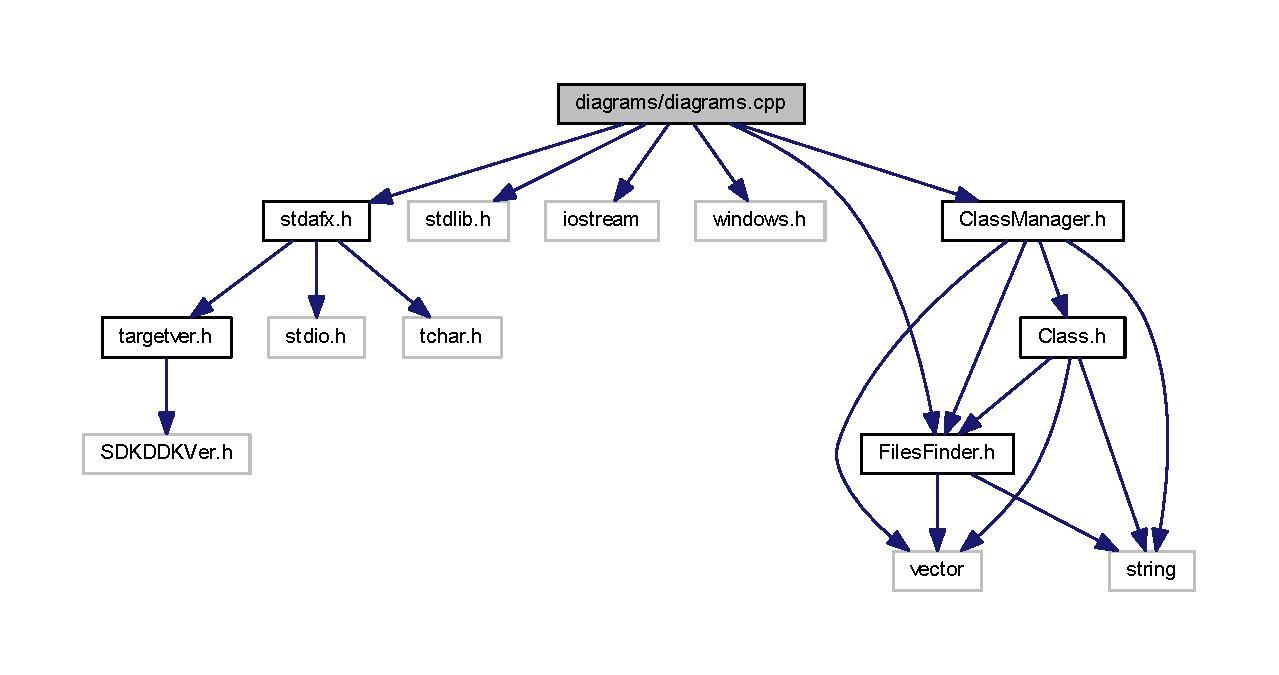
\includegraphics[width=350pt]{diagrams_8cpp__incl}
\end{center}
\end{figure}
\subsection*{Functions}
\begin{DoxyCompactItemize}
\item 
int \hyperlink{diagrams_8cpp_a353674c5af92be7fb389265cde4e5e03}{\+\_\+tmain} (int argc, \+\_\+\+T\+C\+H\+A\+R $\ast$argv\mbox{[}$\,$\mbox{]})
\end{DoxyCompactItemize}


\subsection{Function Documentation}
\hypertarget{diagrams_8cpp_a353674c5af92be7fb389265cde4e5e03}{\index{diagrams.\+cpp@{diagrams.\+cpp}!\+\_\+tmain@{\+\_\+tmain}}
\index{\+\_\+tmain@{\+\_\+tmain}!diagrams.\+cpp@{diagrams.\+cpp}}
\subsubsection[{\+\_\+tmain}]{\setlength{\rightskip}{0pt plus 5cm}int \+\_\+tmain (
\begin{DoxyParamCaption}
\item[{int}]{argc, }
\item[{\+\_\+\+T\+C\+H\+A\+R $\ast$}]{argv\mbox{[}$\,$\mbox{]}}
\end{DoxyParamCaption}
)}}\label{diagrams_8cpp_a353674c5af92be7fb389265cde4e5e03}


Here is the call graph for this function\+:
\nopagebreak
\begin{figure}[H]
\begin{center}
\leavevmode
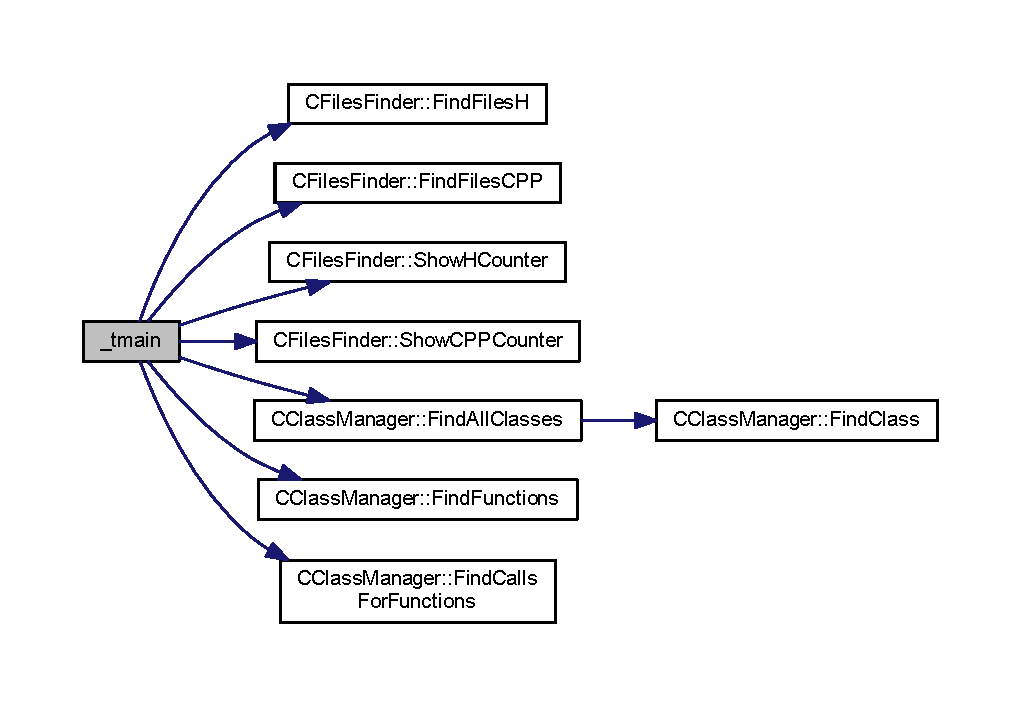
\includegraphics[width=350pt]{diagrams_8cpp_a353674c5af92be7fb389265cde4e5e03_cgraph}
\end{center}
\end{figure}



\hypertarget{_files_finder_8cpp}{\section{diagrams/\+Files\+Finder.cpp File Reference}
\label{_files_finder_8cpp}\index{diagrams/\+Files\+Finder.\+cpp@{diagrams/\+Files\+Finder.\+cpp}}
}
{\ttfamily \#include \char`\"{}stdafx.\+h\char`\"{}}\\*
{\ttfamily \#include \char`\"{}Files\+Finder.\+h\char`\"{}}\\*
{\ttfamily \#include $<$iostream$>$}\\*
{\ttfamily \#include $<$io.\+h$>$}\\*
{\ttfamily \#include $<$windows.\+h$>$}\\*
Include dependency graph for Files\+Finder.\+cpp\+:
\nopagebreak
\begin{figure}[H]
\begin{center}
\leavevmode
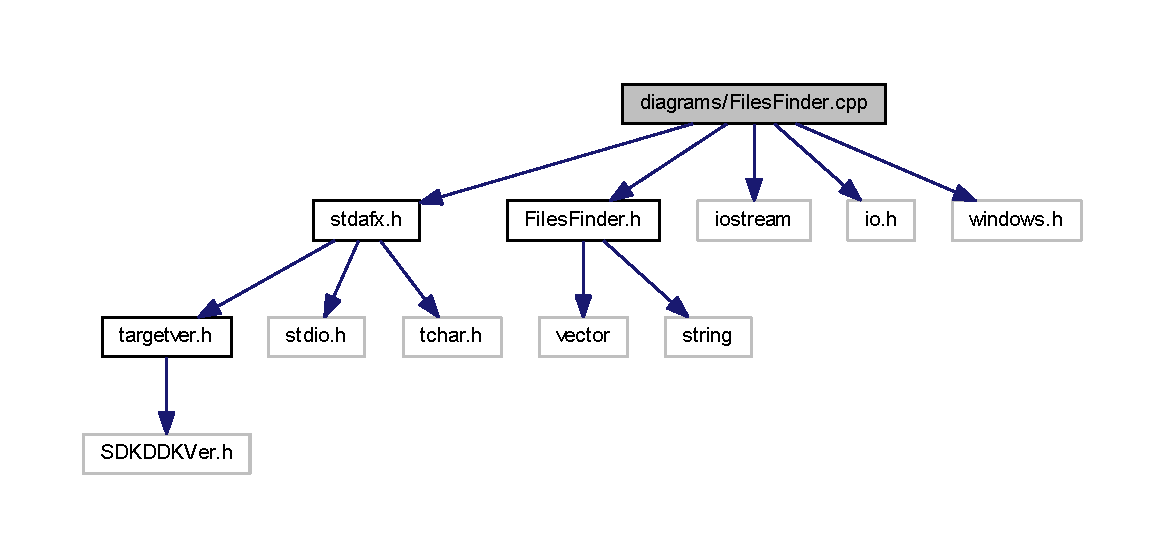
\includegraphics[width=350pt]{_files_finder_8cpp__incl}
\end{center}
\end{figure}

\hypertarget{_files_finder_8h}{\section{diagrams/\+Files\+Finder.h File Reference}
\label{_files_finder_8h}\index{diagrams/\+Files\+Finder.\+h@{diagrams/\+Files\+Finder.\+h}}
}
{\ttfamily \#include $<$vector$>$}\\*
{\ttfamily \#include $<$string$>$}\\*
Include dependency graph for Files\+Finder.\+h\+:
\nopagebreak
\begin{figure}[H]
\begin{center}
\leavevmode
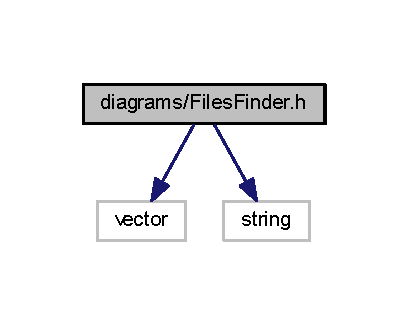
\includegraphics[width=196pt]{_files_finder_8h__incl}
\end{center}
\end{figure}
This graph shows which files directly or indirectly include this file\+:
\nopagebreak
\begin{figure}[H]
\begin{center}
\leavevmode
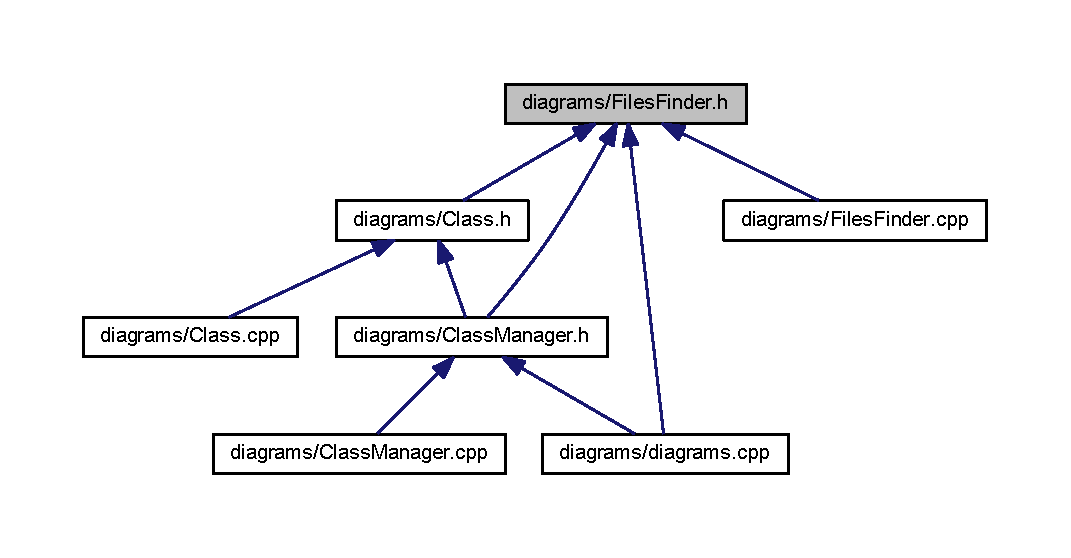
\includegraphics[width=350pt]{_files_finder_8h__dep__incl}
\end{center}
\end{figure}
\subsection*{Classes}
\begin{DoxyCompactItemize}
\item 
class \hyperlink{class_c_files_finder}{C\+Files\+Finder}
\item 
struct \hyperlink{struct_c_files_finder_1_1_s_file}{C\+Files\+Finder\+::\+S\+File}
\end{DoxyCompactItemize}

\hypertarget{stdafx_8cpp}{\section{diagrams/stdafx.cpp File Reference}
\label{stdafx_8cpp}\index{diagrams/stdafx.\+cpp@{diagrams/stdafx.\+cpp}}
}
{\ttfamily \#include \char`\"{}stdafx.\+h\char`\"{}}\\*
Include dependency graph for stdafx.\+cpp\+:
\nopagebreak
\begin{figure}[H]
\begin{center}
\leavevmode
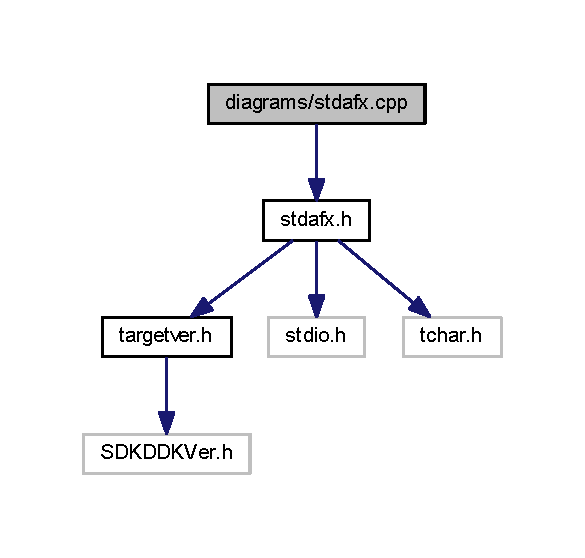
\includegraphics[width=281pt]{stdafx_8cpp__incl}
\end{center}
\end{figure}

\hypertarget{stdafx_8h}{\section{diagrams/stdafx.h File Reference}
\label{stdafx_8h}\index{diagrams/stdafx.\+h@{diagrams/stdafx.\+h}}
}
{\ttfamily \#include \char`\"{}targetver.\+h\char`\"{}}\\*
{\ttfamily \#include $<$stdio.\+h$>$}\\*
{\ttfamily \#include $<$tchar.\+h$>$}\\*
Include dependency graph for stdafx.\+h\+:
\nopagebreak
\begin{figure}[H]
\begin{center}
\leavevmode
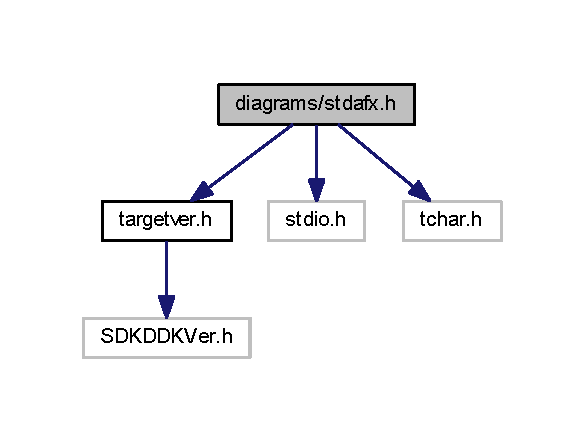
\includegraphics[width=281pt]{stdafx_8h__incl}
\end{center}
\end{figure}
This graph shows which files directly or indirectly include this file\+:
\nopagebreak
\begin{figure}[H]
\begin{center}
\leavevmode
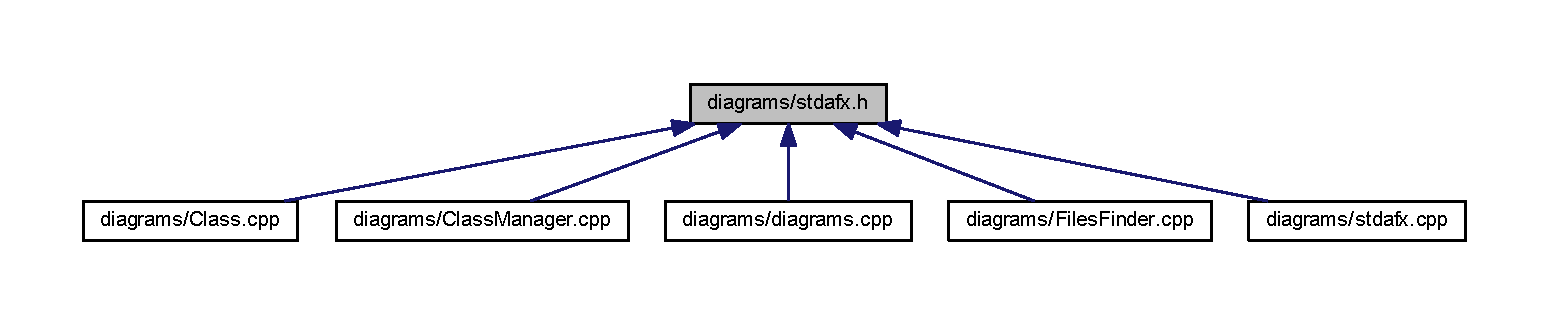
\includegraphics[width=350pt]{stdafx_8h__dep__incl}
\end{center}
\end{figure}

\hypertarget{targetver_8h}{\section{diagrams/targetver.h File Reference}
\label{targetver_8h}\index{diagrams/targetver.\+h@{diagrams/targetver.\+h}}
}
{\ttfamily \#include $<$S\+D\+K\+D\+D\+K\+Ver.\+h$>$}\\*
Include dependency graph for targetver.\+h\+:
\nopagebreak
\begin{figure}[H]
\begin{center}
\leavevmode
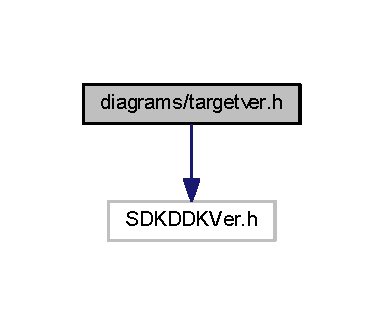
\includegraphics[width=184pt]{targetver_8h__incl}
\end{center}
\end{figure}
This graph shows which files directly or indirectly include this file\+:
\nopagebreak
\begin{figure}[H]
\begin{center}
\leavevmode
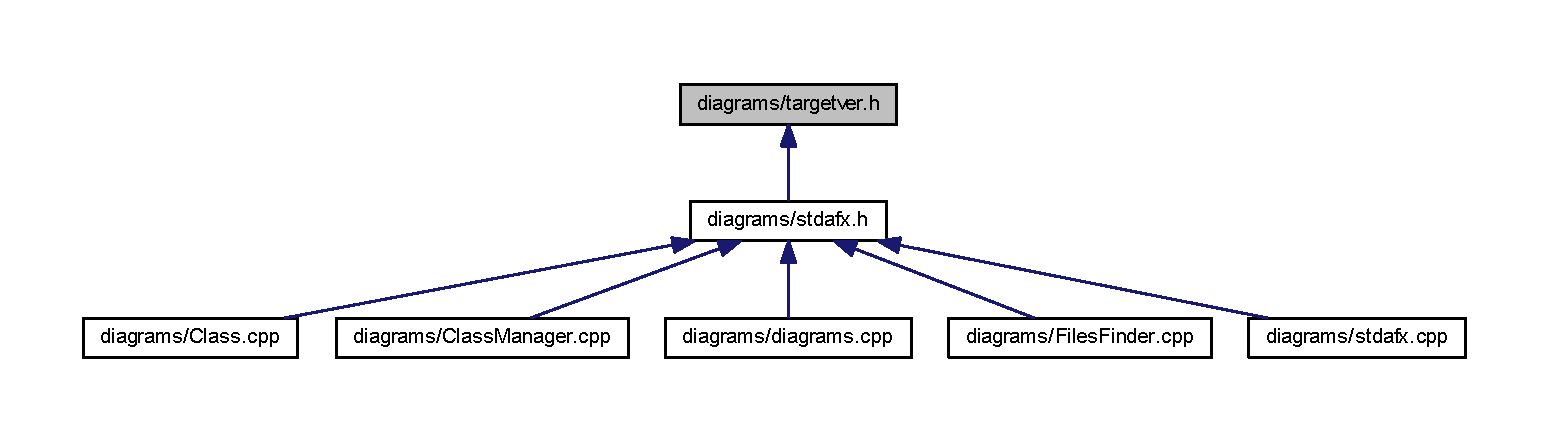
\includegraphics[width=350pt]{targetver_8h__dep__incl}
\end{center}
\end{figure}

%--- End generated contents ---

% Index
\newpage
\phantomsection
\addcontentsline{toc}{chapter}{Index}
\printindex

\end{document}
